%%%%%%%%%%%%%%%%%%%%%%% file template.tex %%%%%%%%%%%%%%%%%%%%%%%%%
%
% This is a general template file for the LaTeX package SVJour3
% for Springer journals.          Springer Heidelberg 2010/09/16
%
% Copy it to a new file with a new name and use it as the basis
% for your article. Delete % signs as needed.
%
% This template includes a few options for different layouts and
% content for various journals. Please consult a previous issue of
% your journal as needed.
%
%%%%%%%%%%%%%%%%%%%%%%%%%%%%%%%%%%%%%%%%%%%%%%%%%%%%%%%%%%%%%%%%%%%
%
% First comes an example EPS file -- just ignore it and
% proceed on the \documentclass line
% your LaTeX will extract the file if required
%
\RequirePackage{fix-cm}
%
%\documentclass{svjour3}                     % onecolumn (standard format)
%\documentclass[smallcondensed]{svjour3}     % onecolumn (ditto)
%\documentclass[smallextended]{svjour3}       % onecolumn (second format)
\documentclass[twocolumn]{svjour3}          % twocolumn
%
\smartqed  % flush right qed marks, e.g. at end of proof
%
\usepackage{graphicx}
\usepackage{amsmath}
\usepackage{amssymb}
\usepackage{subfig}
\usepackage{caption}
\usepackage{cite}
\usepackage{filecontents}
\usepackage{listings}
\usepackage{mathtools, cuted}
\usepackage{tikz}
\usepackage{algorithm}
\usepackage{algpseudocode}
\usetikzlibrary{calc,arrows,shapes,automata,petri,positioning,decorations.markings,shadows}

\usepackage{todonotes}

%\newtheorem{theorem}{Theorem}[section]
\newtheorem{myprop}[theorem]{Proposition}
% \newenvironment{proof}[1][Proof]{\begin{trivlist}
% \item[\hskip \labelsep {\bfseries #1}]}{\end{trivlist}}
\newenvironment{mydef}[1][Definition]{\begin{trivlist}
\item[\hskip \labelsep {\bfseries #1}]}{\end{trivlist}}
\newenvironment{myth}[1][Theorem]{\begin{trivlist}
\item[\hskip \labelsep {\bfseries #1}]}{\end{trivlist}}

\def\pprec{\mathrel{\scalebox{.9}[1]{$\prec$}\mkern-3mu%
  \scalebox{.4}[1]{$\prec$}\mkern-5.5mu\scalebox{.4}[1]{$\prec$}}}
%
% \usepackage{mathptmx}      % use Times fonts if available on your TeX system
%
% insert here the call for the packages your document requires
%\usepackage{latexsym}
% etc.
%
% please place your own definitions here and don't use \def but
% \newcommand{}{}
%
% Insert the name of "your journal" with
% \journalname{myjournal}
%
\begin{document}

\title{The Multi-Stencil Language}
%\subtitle{Do you have a subtitle?\\ If so, write it here}

%\titlerunning{Short form of title}        % if too long for running head

\author{Helene Coullon         \and
        Chirtsian Perez \and
        Julien Bigot
}

%\authorrunning{Short form of author list} % if too long for running head

\institute{Helene Coullon \and Christian Perez \at
              INRIA \\
              46 Allée d'Italie\\
              69007 Lyon\\
              \email{helene.coullon@inria.fr}
           \and
           Julien Bigot \at
           Maison de la Simulation, CEA, CNRS, Univ. Paris-Sud, UVSQ, Universit\'e Paris-Saclay, 91191 Gif-sur-Yvette, France\\
           \email{julien.bigot@cea.fr}
}

%\date{Received: date / Accepted: date}
% The correct dates will be entered by the editor


\maketitle

\begin{abstract}
Insert your abstract here.
\keywords{First keyword \and Second keyword \and More}
\end{abstract}

%------------------------------------------------------------------------------
\section{Introduction}
\label{sect:introduction}
Contributions :
\begin{itemize}
\item Formalism of a multi-stencil program and its parallelization
\item The Multi-stencil Language: agnostic from the type of mesh and of the choosen implementation
\item A first implementation of the MSL compiler (static scheduling + fusion + dump to SkelGIS/components)
\item Evaluation of the different types of parallelism introduced + compiler + fusion
\end{itemize}
%------------------------------------------------------------------------------
\section{Computational model of Multi-Stencil Programs}
\label{sect:formalism}
To numerically solve a set of PDEs, iterative methods (finite difference, finite volume or finite element methods) are frequently used to approximate the solution through a discretized (step by step) phenomena. Thus, the continuous time and space domains are discretized so that a set of numerical computations are iteratively (time discretization) applied onto a mesh (space discretization). In other words, the PDEs are transformed to a set of numerical computations applied at each time step on elements of the discretized space domain. Among those numerical computations are found a set of numerical schemes, also called \textit{stencil computations}, a set of auxiliary computations also called \emph{local computations}, and finally a set of \emph{reductions} to reduce a bunch of values to a single scalar value.
This section gives formal definitions of what we call a \textit{stencil program} and its computations. Then, the different mid-grain parallelization techniques which can be applied on such program, are presented.

We denote stencil kernels discretized explicit numerical schemes which involve neighborhood computations, whatever the type of space discrtization is (mesh).

%-------------------------------------
\subsection{Time, mesh and data}

$\Omega=\mathbb{R}^n$ is the continuous space domain of a numerical simulation. %For example, if $n=3$, any geographic point on earth could be represented in this space in a given geographic coordinate system.
A mesh $\mathcal{M}$ defines the discretization of the continuous space domain $\Omega$ of a set of PDEs and is defined as follows.

\begin{mydef}
A mesh is a connected undirected graph $\mathcal{M}=(V,E)$, where $V\subset \Omega$ is the set of vertices and $E\subseteq V^2$ the set of edges. The set of edges $E$ of a mesh $\mathcal{M}=(V,E)$ does not contain bridges. It is said that the mesh is applied onto $\Omega$.
\end{mydef}
\begin{figure}[!h]\begin{center}
  \resizebox{8cm}{!}{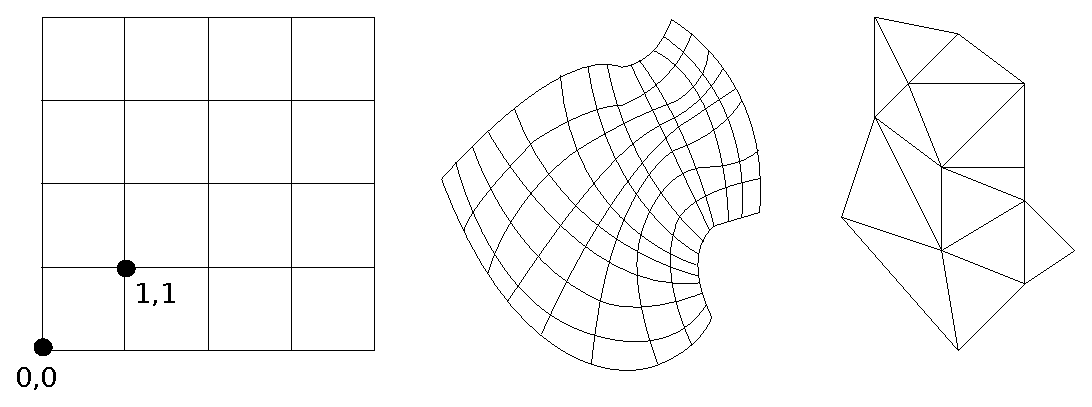
\includegraphics{./images/maillages.pdf}}
  \caption{From left to right, Cartesian, curvilinear and unstructured meshes.}
  \label{fig:mesh}
\end{center}\end{figure}
\begin{mydef}
The dimension of a mesh $\mathcal{M}=(V,E)$ applied onto $\Omega=\mathbb{R}^n$ is denoted $dim(\mathcal{M})=n$.
\end{mydef}
A mesh can be structured (as Cartesian or curvilinear meshes), unstructured, regular or irregular (without the same topology for each element) and hybrid as illustrated in Figure~\ref{fig:mesh}.

\medskip
\noindent \textbf{Definitions}
%\begin{mydef}
\begin{itemize}
\item An entity $e$ of a mesh $\mathcal{M}=(V,E)$ is defined as a subset of its vertices and edges, $e\subset V\cup E$.
\item A group of mesh entities is denoted $E$ such that $E \in \mathcal{P}(V\cup E)$. It represents a set of entities of the same type.
\item The set of mesh entities groups of a simulation is denoted $\mathcal{E}$.
\item Finally, the mesh on which is applied a group of mesh entities $E$ is denoted $mesh(E)$
\end{itemize}
%\end{mydef}

For example, in a 2D Cartesian mesh an entity could be a cell, made of four vertices and four edges, or simply a vertex. As a result, a group of cells and a group of vertices could be defined in $\mathcal{E}$. %This type can be defined as the sets containing exactly four vertices and four edges connected as a cycle. Another type of entities simply are the vertices ($V$) and can be defined as all singletons formed of a single vertex of $V$.

\medskip
This covers the space discretization, however there is also the time dimension which has to be discretized in the simulation.

\medskip
\noindent \textbf{Definitions}
%\begin{mydef}
\begin{itemize}
\item We denote a scalar as an identifier associated to a numerical value and applied onto a mesh $\mathcal{M}$ where $dim(\mathcal{M})=0$. In other words a scalar can be seen as a variable containing a numerical value. The set of scalars is denoted $\mathcal{S}$.
\item $\mathcal{T}=\mathbb{R}$ is the continuous time domain of a numerical simulation.
\item The discretization of the continuous time domain $\mathcal{T}$ is denoted as the pair $T(\Delta t,conv)$.
\begin{itemize}
\item $\Delta t \in \mathcal{S}$ represents the time interval of the numerical simulation, such that for a current time iteration $t_i$, the next time iteration is $t_{i+1} = t_i + \Delta t$. The default value of $\Delta t$ is $1$.
\item $conv:\mathcal{S}^n \rightarrow bool$ is a function which returns a boolean from a set of scalar variables. This function represents the convergence criteria of the simulation. 
\item At a given time step, the convergence criteria is evaluated such that if $conv$ returns $true$ the next time step can start such that $t_{i+1} = t_i + \Delta t$, otherwise the simulation ends. For example, the simplest $conv$ is typically to have two scalars: $t$ the time, and a fix number of iterations denoted $it$. At each time step $\Delta t=1$, and $conv$ returns the boolean expression $t<it$.
\end{itemize}
\end{itemize}
%\end{mydef}

%$T$ is responsible for the iteration time steps of the numerical simulation. A numerical simulation though does not run forever and must be stopped at some point. Some simulations choose a fix number of time iteration, others compute a \emph{convergence} criteria at the end of each time iteration to determine if the simulation has to continue. A convergence criteria is computed by a reduction computation that will be detailed in the next section.

In a numerical simulation, as a set of scalars can be applied onto a mesh with a nil dimension, a set of data elements, or quantities, can be applied onto meshes of dimension superior to zero. Those quantities represent, as well as scalars, the set of values to compute, or to use, for computations.

\medskip
\noindent \textbf{Definitions}
%\begin{mydef}
\begin{itemize}
\item A quantity (or data) is a function $\delta: E_{\delta} \mapsto V_{\delta}$ which associates each entity of a group $e\in E_{\delta}$ to a value $v\in V_{\delta}$ where $V_{\delta}$ is a primitive data type, typically $\mathbb{R}$, $\mathbb{N}$ or $\mathbb{C}$.
\item The set of quantities applied onto the mesh is denoted $\Delta$.
\item In the rest of this paper, the group of mesh entities on which a quantity $\delta$ is mapped is denoted $entity(\delta)=E_{\delta}$.
\end{itemize}
%\end{mydef}

Another option, closer to the applied mathematics domain, would have been to define $\delta$ as the function over $E_{\delta} \times T$. In this case a single quantity would represents all its occurences over time steps. This solution could be investigated in future work, however the approach chosen for now is to let the user be aware of the number of data he is using and what exactly for.

%-----------------------
\subsection{Computations}

In this section are considered four different types of kernel computations, stencil kernels, boundary kernels, local kernels, and reduction kernels. 

\medskip
\noindent \textbf{Definitions}
%\begin{mydef}
\begin{itemize}
\item A computation domain $D$ is a subpart of a mesh entities group, $D \subseteq E \in \mathcal{E}$.
\item The set of computation domains of a numerical simulation is denoted $\mathcal{D}$.
\item A neighborhood $n$ is a function which for a given entity $e \in E_i$, returns a set of $m$ entities in $E_j$, $n : E_i \rightarrow E_j^m$. One can notice that $i = j$ is possible. Most of the time, such a neighborhood is called a stencil shape.
\item The set of neihborhood functions in a numerical simulation is denoted $\mathcal{N}$.
\end{itemize}

\begin{mydef}
A computation kernel $k$ of a numerical simulation is defined as $k(S,R,(w,D),comp)$, where 
\begin{itemize}
\item $S \in \mathcal{S}$ is the set of scalar to read, 
\item $(w,D) \in \Delta \times \mathcal{D}$ is the single data modified by the computation kernel onto a given computation domain. Thus, $w \in \Delta$ and $D \in \mathcal{D}$ is the computation domain on which $w$ is computed, $D \subseteq E_w=entity(w)$.
\item $R$ is the set of tuples $(r,n)$, where $r \in \Delta$ and $n \in \mathcal{N}$ is a neighborhood function such that $n : E_w \rightarrow entity(r)^m$. The neighborhood indicates which entities of $r$ will be read in order to compute a single entity of $w$. 
\item $comp$ is the numerical computation which returns a value from a set of $n$ input values, $comp: V^n \rightarrow V$.
\end{itemize}
% \item A numerical expression $\text{exp}_{w}: entity(w) \times R^n \rightarrow V_{w}$ is a function which computes the values of the written quantity $w \in \Delta$ for a given entity $e \in entity(w)=E_w$, using a set of input data $R$.
% \item A computation kernel $k$ of a numerical simulation is defined as $c(R,w,\text{exp},D)$, where $R$ is the set of data read, $w \in \Delta$ is the unique data written, $\text{exp}$ is a numerical expression, and $D \in \mathcal{D}$ is the computation domain.
% \end{itemize}
%$R$ is the set of data read, $w \in \Delta$ is the unique data written, $\text{exp}$ is a numerical expression, and $D \in \mathcal{D}$ is the computation domain.
\end{mydef}

$comp$ represents the actual numerical expression which is computed by a kernel. We can dissociate four types of kernel computations.

\noindent \textbf{Definitions}
%\begin{mydef}
\begin{itemize}
\item We denote by $identity$ the identity function $x=x$.
\item A kernel computation $k(S,R,(w,D),comp)$ is a \emph{stencil kernel} $\iff \exists (r,n) \in R$ such that $n \neq identity$ and if $\exists (r,n)$ with $r=w$ then $n=identity$.
\item A kernel computation $k(S,R,(w,D),comp)$ is a \emph{boundary kernel} $\iff \exists (r,n) \in R$ such that $r=w$ and such that $n \neq identity$.
\item A kernel computation $k(S,R,(w,D),comp)$ is a \emph{local kernel} $\iff \forall (r,n) \in R$, $n = identity$.
\item A kernel computation $k(S,R,(w,D),comp)$ is a \emph{reduction kernel} $\iff w$ is a scalar, $R=\{(r,n)\}$, and if $n=entity(r)$.
\end{itemize}

In our formalism, it is forbidden for a stencil kernel to find $(r,n) \in R$ for which $r=w$ and $n \neq identity$. Actually, if such a property was permitted, implicit numerical schemes would be needed into the simulation, which involves linear solvers. Such a scheme is not a stencil and is over the scope of this paper. The problem does not happened for local kernels as $\forall (r,n) \in R$, $n = identity$. Computations for which this property is authorized are boundary kernels only. This type of kernel is a particular case as it commputes boundary conditions, which represents what should happened outside the space domain but still impact stencil kernels at the next time step.

\noindent \textbf{Property}
A kernel for which all data read and written are applied onto a mesh of dimension $0$ is a local kernel.

\noindent \textbf{Property}
In a reduction kernel $k(S,R,(w,D),comp)$, $D=entity(w)$ as a single entity exists for a scalar.

\medskip
A reduction computation is a computation which reads a single data applied onto a mesh and returns from all its entities a single scalar (mesh with a dimension reduced to zero). A reduction is typically used to compute the convergence criteria of the time loop of the simulation. Occasionally reductions can also be used during a time iteration. %This last usage is typically done to have a conditionnal branch to choose one computation or another, or to compute a dynamic time step for example.

\medskip
\noindent \textbf{Property}
Considering a reduction kernel $k(S,R,(w,D),comp)$, $comp$ must be a binary and associative operation on the type $V$, $comp: V \times V \rightarrow V$.

\medskip
\noindent \textbf{Definitions}
\begin{itemize}
\item The set of $n$ ordered computation kernels of a numerical simulation is denoted $\Gamma = [k_i]_{0 \leq i \leq n-1}$, such that $\forall k_i,k_j \in \Gamma$, if $i < j$, then $k_i$ is computed before $k_j$.
\item Finally, a \textit{multi-stencil program} is defined by the octuplet 
\begin{equation*}
\mathcal{MSP}(T,\mathcal{M},\mathcal{E},\mathcal{D},\mathcal{N},\Delta, \mathcal{S},\Gamma)
\end{equation*}
\end{itemize}

For example, in Figure~\ref{fig:ex1}, assuming that the computation domain (full lines) is denoted $dc1$ and the stencil shape is $n1$, the stencil kernel can be defined as:
\begin{equation*}
R: \{(B,n1)\}, \quad w: A, \quad D: dc1,
\end{equation*}
\begin{equation*}
comp: A(x,y)=B(x+1,y)+B(x-1,y)+B(x,y+1)+B(x,y-1).
\end{equation*}
On the other hand, in the example of Figure~\ref{fig:ex2}, assuming the computation domain is $dc2$ and the stencil shape is $n2$, the stencil kernel is defined as:
\begin{equation*}
R: \{(C,n2),(A,identity)\}, \quad w: A, \quad D: dc2,
\end{equation*}
\begin{equation*}
comp: A(x,y)=A(x,y)+C(x1,y1)+C(x1+1,y1).
\end{equation*}

\begin{figure}
\begin{center}
\subfloat[Mesh and mesh domains.\label{fig:meshbase}]{
\resizebox{8cm}{!}{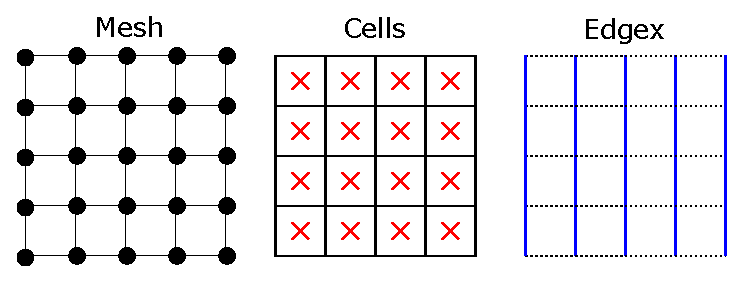
\includegraphics{./images/mesh.pdf}}
}\\
\hspace{10pt}
\subfloat[4-neighborhood stencil.\label{fig:ex1}]{
\resizebox{5cm}{!}{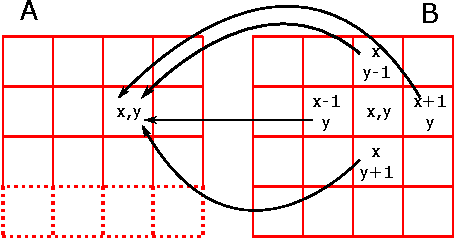
\includegraphics{./images/stencil1.pdf}}
}
\vspace{20pt}
\subfloat[4-neighborhood stencil.\label{fig:ex2}]{
\resizebox{5cm}{!}{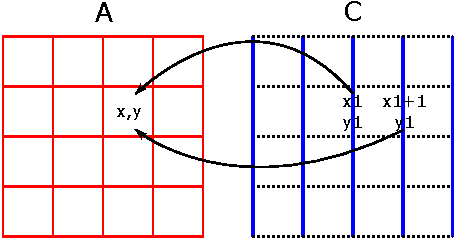
\includegraphics{./images/stencil2.pdf}}
}
\end{center}
\caption{(a) a Cartesian mesh and two kind of mesh entities, (b) an example of stencil kernel on cells, (c) an example of stencil kernel on two different entities of the mesh.}
\label{fig:gspmsp}
\end{figure}

A stencil program has been formally defined in this section. This formalism is used in the next Section to define two parallelization techniques of a multi-stencil program.

One can note that all definitions given in this section are not dependent from the topology of the mesh. This property will be kept in the rest of this paper to propose the mesh-agnostic MSL language.



% Formalism :
% \begin{itemize}
% \item mesh / mesh entities and groups / computations domains
% \item data and scalars
% \item computations : stencil, local and reduction
% \item Multi-Stencil Program
% \end{itemize}
%------------------------------------------------------------------------------
\section{Parallelization of Multi-Stencil Programs}
\label{sect:parallelism}
% Multi-stencil mesh-based numerical simulation can be parallelized in various ways and is an interesting kind of application to take advantage of modern heterogeneous HPC architectures, mixing clusters, multi-cores CPUs, vectorization units, GPGPU and many-core accelerators.
As previously explained, in a computation $k(S,R,(w,D),comp)$, $comp$ is not handled by MSL. As a result, in the rest of this paper, and to simplify notations, we denote the same computation $k(S,R,(w,D))$.

%------------------------------
\subsection{Data parallelism}
\label{sect:dataparal}
In a data parallelization technique, the idea is to split quantities on which the program is computed into balanced sub-parts, one for each available resource. The same sequential program can afterwards be applied on each sub-part simultaneously, with some additioinal synchronizations between resources to update the data not computed locally, and thus to guarantee a correct result.

\medskip
More formally, the data parallelization of a multi-stencil program 
\begin{equation*}
\mathcal{MSP}(\mathcal{M},\Phi,\mathcal{D},\mathcal{N},\Delta, \mathcal{S},T,\Gamma)
\end{equation*}

consists in, first, a partitioning of the mesh $\mathcal{M}$ in $p$ balanced sub-meshes (for $p$ resources) $\mathcal{M}=\{\mathcal{M}_0,\dots,\mathcal{M}_{p-1}\}$. This step can be performed by an external graph partitionner~\cite{} and is not adressed by this paper. 

As entities and quantities are mapped onto the mesh, the set of groups of mesh entities and the set of quantities $\Delta$ are partitionned the same way than the mesh: $\Phi=\{\Phi_0,\dots,\Phi_{p-1}\}$, $\Delta=\{\Delta_0,\dots,\Delta_{p-1}\}$. 

The second step of the parallelization is to identify in $\Gamma$ the needed synchronizations between resources to update data, and thus to build a new ordered list of computations $\Gamma_{sync}$.

\begin{mydef}
For $n$ the number of computations in $\Gamma$, and for $i,j$ such that $i<j<n$, a \textit{synchronization} is needed between $k_i$ and $k_j$, denoted $k_i \pprec k_j$, if $\exists (r_j,n_j) \in R_j$ such that $w_i=r_j$ and $n_j\neq identity$ ($k_j$ is a stencil computation). The quantity to synchronize is $\{w_i\}$.
\label{def:sync}
\end{mydef}

Actually, a synchronization is needed by the quantity read by a stencil computation (not local), if this quantity has been modified before, which means that it has been written before. This synchronization is needed because a neighborhood function $n \in \mathcal{N}$ of a stencil computation involves values computed on different resources.

However, as a multi-stencil program is an iterative program, computations which happen after $k_j$ at the time iteration $t$ have also been computed before $k_j$ at the previous time iteration $t-1$. For this reason another case of synchronization has to be defined.

\begin{mydef}
For $n$ the number of computations in $\Gamma$ and $j<n$, if $\exists (r_j,n_j) \in R_j$ such that $n_j\neq identity$ and for all $i<j$, $k_i \not \pprec k_j$, a \textit{synchronization} is needed between $k_l$ and $k_j$, where $j<l<n$, denoted $k_l \pprec k_j$, if $w_l=r_j$. The quantity to synchronize is $\{w_l\}$.
\label{def:sync2}
\end{mydef}

\begin{mydef}
A synchronization between two computations $k_i \pprec k_j$ is defined as a specific computation 
\begin{equation*}
k_{i,j}^{sync}(S,R,(w,D)), 
\end{equation*}
where $S=\emptyset$, $R=\{(r,n)\}=\{(w_i,n_j \in \mathcal{N}\}$, $(w,D)=(w_i,\bigcup_{\phi \in D_j} n_j(\phi)))$. In other words, $w_i$ has to be synchronized for the neighborhood $n_j$ for all entities of $D_j$.
\end{mydef}

\begin{mydef}
If $k_i \pprec k_j$, $k_j$ is replaced by the list
\begin{equation*}
[k_{i,j}^{sync}, k_j]
\end{equation*}
\end{mydef}

When data parallelism is applied, the other type of computation which is responsible for additional synchronizations is the reduction. Actually, the reduction is first applied locally on each subset of entities, on each resource. Thus, $p$ (number of resources) scalar values are obtained. For this reason, to perform the final reduction, a set of synchronizations are needed to get the final reduced scalar. As most parallelism libraries (MPI, OpenMP) already propose a reduction synchronization with its own optimizations, we simply choose to replace the reduction computation by itself anotated by $red$.

\begin{mydef}
A reduction kernel $k_j(S_j,R_j,(w_j,D_j))$, where $w$ is a scalar, is replaced by $k^{red}_j(S_j,R_j,(w_j,D_j))$. %if we denote by $w^r$, $0 \leq r<p$, the local scalar $w$ computed on the resource $r$, a reduction synchronization is defined as the specific computation 
% \begin{equation*}
% k_{j}^{sync}(S,R,(w,D),comp)
% \end{equation*}
\label{def:red}
\end{mydef}
% where, $S=\emptyset$, $R=\{(w^0,entity(w^0)) \dots (w^{p-1},entity(w^{p-1}))\}$, and $w=w_i$, $D=entity(w)=D_i$ and $comp=comp_i$.

One can notice that both types of synchronizations are performed by all resources.

\begin{mydef}
The concatenation of two ordered lists of respectively $n$ and $m$ computations $l_1=[k_i]_{0 \leq i \leq n-1}$ and $l_2=[k'_i]_{0 \leq i \leq m-1}$ is denoted $l_1 \cdot l_2$ and is equal to a new ordered list $l_3=[k_0,\dots,k_{n-1},k'_0,\dots,k'_{m-1}]$.
\end{mydef}

\begin{mydef}
From the ordered list of computation $\Gamma$, a new synchronized ordered list $\Gamma_{sync}$ is obtained from the call $\Gamma_{sync} = F_{sync}(\Gamma,0)$, where $F_{sync}$ is the recursive function defined in Algorithm~\ref{alg:sync}.
\end{mydef}

Algorithm~\ref{alg:sync} follows previous definitions to build a new ordered list which includes synchronizations. In this algorithm, lines 7 to 19 apply Definition~(\ref{def:sync}), lines 20 to 29 apply Definition~(\ref{def:sync2}), and finally lines 34 and 35 apply Definition~(\ref{def:red}). Finally, line 39 of the algorithm is the recursive call.

\begin{algorithm}
\caption{$F_{sync}$ recursive function}
\label{alg:sync}
\begin{algorithmic}[1]
\Procedure{$F_{sync}$} {$\Gamma$,$j$}
\State $k_j = \Gamma[j]$
\State $list = []$
\If {$j=|\Gamma|$}
\State return $list$
\ElsIf {$\exists (r_j,n_j) \in R_j$ such that $n_j\neq identity$}
\For {all $(r_j,n_j) \in R_j$ such that $n_j\neq identity$}
\State found = false
\For {$0 \leq i<j$}
\State $k_i = \Gamma[i]$
\If {$k_i \pprec k_j$}
\State found = true
\State $S = \emptyset$
\State $R = \{(w_i,n_j)\}$
\State $(w,D) = (w_i,\bigcup_{\phi \in D_j} n_j(\phi)))$
%\State $comp = identity$
\State $list.[k_{i;j}^{sync}(S,R,(w,D))]$%,comp)]$
\EndIf
\EndFor
\If {!found}
\For {$j<i\leq n$}
\State $k_i = \Gamma[i]$
\If {$k_i \pprec k_j$}
\State $S = \emptyset$
\State $R = \{(w_i,n_j)\}$
\State $(w,D) = (w_i,\bigcup_{\phi \in D_j} n_j(\phi)))$
%\State $comp = identity$
\State $list.[k_{i;j}^{sync}(S,R,(w,D))]$%,comp)]$
\EndIf
\EndFor
\EndIf
\State $list \cdot [k_j]$
\EndFor
\ElsIf {$w_j \in \mathcal{S}$}
\State $list.[k^{red}_j]$
\Else
\State $list.[k_j]$
\EndIf
\State return $list \cdot F_{sync}(\Gamma,j+1)$
\EndProcedure
\end{algorithmic}
\end{algorithm}


 The final step of this parallelization is to run $\Gamma_{sync}$ on each resource. Thus, for each resource $0 \leq r \leq p-1$ the multi-stencil program 
\begin{equation}
\mathcal{MSP}_r(\mathcal{M}_r,\Phi_r,\mathcal{D}_r,\mathcal{N},\Delta_r,\mathcal{S},T,\Gamma_{sync}),
\end{equation}
is performed.

\paragraph{\textbf{Example}} Figure~\ref{fig:exmsl} gives an example of a $\mathcal{MSP}$ program. From this example, the following ordered list of computation kernels can be extracted:
\begin{equation*}
\Gamma = [k_0,k_1,k_2,k_3,k_4,k_0,k_6,k_7,k_8]
\end{equation*}
From this ordered list of computation kernels $\Gamma$, and from the rest of the multi-stencil program, synchronizations can be automatically detected from the call to $F_{sync}(\Gamma,0)$ to get the synchronized ordered list of kernels:
\begin{equation}
\Gamma_{sync} = [k_0,k_{0;1}^{sync},k_1,k_2,k_3,k_{1;4}^{sync},k_4,k_0,k_6,k_7,k_{7;8}^{sync},k_8],
\label{eq:exsync}
\end{equation}
\begin{subequations}
where
\begin{align}
        k_{0;1}^{sync}=(\emptyset,\{(B,nce)\},(B,\cup_{\phi \in D_1} nce(\phi)),identity),\\
        k_{1;4}^{sync}=(\emptyset,\{(C,nec)\},(C,\cup_{\phi \in D_4} nec(\phi)),identity),\\
        k_{7;8}^{sync}=(\emptyset,\{(I,ncc)\},(I,\cup_{\phi \in D_8} ncc(\phi)),identity).
\end{align}
\end{subequations}

%------------------------------
\subsection{Hybrid parallelism}
A task parallelization technique is a technique to transform a program as a dependency graph of different tasks. A dependency graph exhibits parallel tasks, or on the contrary sequential execution of tasks. Such a dependency graph can directly be given to a dynamic scheduler, or can statically be scheduled. In this paper, we introduce task parallelism by building the dependency graph between kernels of the sequential list $\Gamma_{sync}$. Thus, as $\Gamma_{sync}$ takes into account data parallelism, we introduce hybrid parallelism.

\begin{mydef}
For two computations $k_i$ and $k_j$, with $i < j$, it is said that $k_j$ is dependant from $k_i$ with a \emph{read after write} dependency, denoted $k_i \prec_{raw} k_j$, if $\exists (r_j,n_j) \in R_j$ such that $w_i=r_j$. In this case, $k_i$ has to be computed before $k_j$.
\end{mydef}

\begin{mydef}
For two computations $k_i$ and $k_j$, with $i < j$, it is said that $k_j$ is dependant from $k_i$ with a \emph{write after write} dependency, denoted $k_i \prec_{waw} k_j$, if $w_i = w_j$ and $D_i \cap D_j \neq \emptyset$. In this case, $k_i$ also has to be computed before $k_j$.
\end{mydef}

\begin{mydef}
For two computations $k_i$ and $k_j$, with $i < j$, it is said that $k_j$ is dependant from $k_i$ with a \emph{write after read} dependency, denoted $k_i \prec_{war} k_j$, if $\exists (r_i,n_i) \in R_i$ such that $w_j=r_i$. In this case, $k_i$ also has to be computed before $k_j$ is started so that values read by $k_i$ are relevant.
\end{mydef}

Those definitions are known as \emph{data hazards classification}. However, a specific condition on the computation domain, due to the specific domain of multi-stencils, is introduced for the write after write case.

\begin{mydef}
A directed acyclic graph (DAG) $G(V,A)$ is a graph where the edges are directed from a source to a destination vertex, and where, by following edges direction, no cycle can be found from a vertex $u$ to itself. A directed edge is called an arc, and for two vertices $v,u \in V$ an arc from $u$ to $v$ is denoted $(\overset{\frown}{u,v}) \in A$.
\end{mydef}

From an ordered list of computations $\Gamma_{sync}$, a directed dependency graph $\Gamma_{dep}(V,A)$ can be built finding all pairs of computations $k_i$ and $k_j$, with $i<j$, such that $k_i \prec_{raw} k_j$ or $k_i \prec_{waw} k_j$ or $k_i \prec_{war} k_j$. 

\begin{mydef}
For two directed graphs $G(V,A)$ and $G'(V',A')$, the union $(V,A)\cup (V',A')$ is defined as the union of each set $(V\cup V', A \cup A')$.
\end{mydef}

\begin{mydef}
From the synchronized ordered list of computation kernels $\Gamma_{sync}$, the dependency graph of the computations $\Gamma_{dep}(V,A)$ is obtained from the call $F_{dep}(\Gamma_{sync},0)$, where $F_{dep}$ is the recursive function defined in Algorithm~\ref{alg:dep}.

% \begin{equation*}
% F_{dep}(\Gamma_{sync},j) = 
% \begin{cases} 	\bullet (\{\},\{\}) \mbox{ if }j=|\Gamma_{sync}|\\
% 				\bullet (k_j, \{(\overset{\frown}{k_i,k_j})\mbox{, }\forall i < j \mbox{, } k_i\prec k_j \})\\
% 				\text{ } \qquad \cup F_{dep}(\Gamma_{sync},j+1) \mbox{ if }j<|\Gamma_{sync}|
% \end{cases}
% \end{equation*}
\end{mydef}

\begin{algorithm}
\caption{$F_{dep}$ recursive function}
\label{alg:dep}
\begin{algorithmic}[1]
\Procedure{$F_{dep}$} {$\Gamma_{sync}$,$j$}
\State $k_j = \Gamma_{sync}[j]$
\If {$j=|\Gamma_{sync}|$}
\State return $(\{\},\{\})$
\ElsIf {$j<|\Gamma_{sync}|$}
\State $G=(\{\},\{\})$
\For {$0 \leq i<j$}
\State $k_i = \Gamma_{sync}[i]$
\If {$k_i \prec_{raw} k_j$ or $k_i \prec_{waw} k_j$ or $k_i \prec_{war} k_j$}
\State $G = G \cup (k_j, \{(\overset{\frown}{k_i,k_j} \})$
\EndIf
\EndFor
\State return $G \cup F_{dep}(\Gamma_{sync},j+1)$
\EndIf
\EndProcedure
\end{algorithmic}
\end{algorithm}

This constructive function is possible because the input is an ordered list. Actually, if $k_i\prec k_j$ then $i<j$. As a result, $k_i$ is already in $V$ when the arc $(\overset{\frown}{k_i,k_j})$ is built.

One can notice that $\Gamma_{dep}$ is the dependency graph of the computations of a multi-stencil program, but it only takes into account a single time iteration. A complete dependency graph of the simulation could be built. This is a possible extension of this work.

\begin{myprop}
The directed graph $\Gamma_{dep}$ is an acyclic graph.
\end{myprop}

% \begin{proof}
% $\Gamma_{dep}$ is built from $\Gamma_{sync}$ which is an ordered and sequential list of computations. Moreover, each computation of the list $\Gamma_{sync}$ is associated to a vertex of $V$, even if the same computation is represented more than once in $\Gamma_{sync}$. As a result it is not possible to go back to a previous computation and to create a cycle.
% \end{proof}

As a result of the hybrid parallelization, each resource $0 \leq r \leq p-1$ perform a multi-stencil program, defined by
\begin{equation*}
\mathcal{MSP}_r(\mathcal{M}_r,\Phi_r,\mathcal{D}_r,\mathcal{N},\Delta_r,T,\Gamma_{dep}).
\end{equation*}
The set of computations $\Gamma_{dep}$ is a dependency graph between computation kernels $k_i$ of $\Gamma$ and synchronizations of kernels added into $\Gamma_{sync}$. $\Gamma_{dep}$ can be built from the call to 
\begin{equation*}
F_{dep}(F_{sync}(\Gamma,0),0).
\end{equation*}

\paragraph{\textbf{Example}} Figure~\ref{fig:exmsl} gives an example of $\mathcal{MSP}$ program. From $\Gamma_{sync}$ that has been built in Equation~(\ref{eq:exsync}), the dependency DAG can be built. For example, as $k_0$ computes $B$ and $k_1$ reads $B$, $k_0$ and $k_1$ becomes vertices of $\Gamma_{dep}$, and an arc $(\overset{\frown}{k_0,k_1})$ is added to $\Gamma_{dep}$. The overall $\Gamma_{dep}$ built from the call to $F_{dep}(\Gamma_{sync},0)$ is drawn in Figure~\ref{fig:depdep}.
\begin{figure}[h!]
\begin{center}
\begin{tikzpicture}[shorten >=1pt, node distance=2cm, on grid, auto]
   \node[] (c0) at (0,0) {$k_0$};
   \node[] (star1) at (1,0) {$k_{0;1}^{sync}$};
   \node[] (c1) at (2,0) {$k_1$};
   \node[] (c2) at (3,0.5) {$k_2$};
   \node[] (star4) at (3,1.5) {$k_{1;4}^{sync}$};
   \node[] (c3) at (3,-0.5) {$k_3$};
   \node[] (c4) at (4,0.5) {$k_4$};
   \node[] (c5) at (4,-0.5) {$k_5$};
   \node[] (c6) at (5,0.5) {$k_6$};
   \node[] (c7) at (6,0) {$k_7$};
   \node[] (star8) at (7,0) {$k_{7;8}^{sync}$};
   \node[] (c8) at (8,0) {$k_8$};
 
  \path[->]
    (c0) edge node {} (star1)
    (star1) edge node {} (c1)
    (c1) edge node {} (c2)
         edge node {} (c3)
         edge node {} (star4)
    (star4) edge node {} (c4)
    (c2) edge node {} (c4)
    (c4) edge node {} (c6)
    (c3) edge node {} (c5)
    (c5) edge node {} (c7)
    (c6) edge node {} (c7)
    (c7) edge node {} (star8)
    (star8) edge node {} (c8);
  \end{tikzpicture}
\caption{$\Gamma_{dep}$ of the example of program of Figure~\ref{fig:exmsl}}
\label{fig:depdep}
\end{center}
\end{figure}
% Parallelization formalism :
% \begin{itemize}
% \item Data parallelism (introduction of synchronizations)
% \item Task parallelism (computation of the dependency graph)
% \end{itemize}
%------------------------------------------------------------------------------
\section{The Multi-Stencil Language}
\label{sect:msl}
\begin{filecontents*}{grammar.txt}
program ::= "mesh:" meshid 
            "mesh entities:" listmeshent
            "computation domains:" 
                       listcompdom
            "independent:"
                       listinde
            "data:" listdata
            listloop

listmeshent ::= meshent listmeshent |  meshent
listcompdom ::= compdom listcompdom |  compdom
compdom ::= compdomid "in" listmeshent
listinde ::= inde listinde |  inde
inde ::= compdomid "and" compdomid
listdata ::= data listdata |  data
data ::= dataid "," meshent

listloop ::= loop listloop | loop
loop ::=  "time:" iteration
          "reductions:" listred
          "computations:" listcomp
          
iteration ::= num | red
listcomp ::= comp listcomp |  comp
comp ::= dataid "[" compdomid "]=" compid "(" listdataread ")"
listred ::= red listred | red
red ::= redid "(" listdataread ")"
listdataread ::= dataread listdataread |  dataread
dataread ::= dataid "[" neighborid "]" |  dataid
\end{filecontents*}

\begin{figure}[t]
  \hspace{5mm}
  \begin{minipage}[t]{\textwidth}
    %  \subfloat[\label{fig:grammar}]
    {\lstinputlisting[basicstyle=\small,mathescape,frame=single,language=Python,numbers=left,linewidth=.87\textwidth]{grammar.txt}}   
    \caption{Grammar of the Multi-Stencil Language. \label{fig:grammar}}
  \end{minipage}
\end{figure}
The parallel empty skeleton of the application can be computed automatically from the language :
\begin{itemize}
\item grammar
\item example from the language to $\Gamma$
\end{itemize}
%------------------------------------------------------------------------------
\section{Static Scheduling}
\label{sect:msp}
In this section we argue that the graphs $\Gamma_{hybrid}$ or $\Gamma_{task}$, previously defined, on which an approximation will be defined, are minimal series-parallel graphs. For this reason, the structure of those graphs can be represented as binary trees of parallel and series compositions of sub-graphs, also called \emph{binary decomposition tree}~\cite{Valdes:1979:RSP:800135.804393}. First, the needed definitions on series-parallel graphs will be given...

%--------------------
\subsection{GSP and MSP classes}
A vertex $v$ of a DAG $G$ is a \emph{source} if no edge of $G$ enters $v$. Similarly, a vertex $v$ is a \emph{sink} if no edge of $G$ leaves $v$. In 1982, Valdes \& Al~\cite{Valdes:1979:RSP:800135.804393} have defined the class of minimal series-parallel DAGs (MSP).

\begin{mydef}Minimal Series Parallel
\begin{itemize}
\item The DAG having a single vertex and no edges is MSP.
\item If $G_1=(V_1,E_1)$ and $G_2=(V_2,E_2)$ are two MSP DAGs, so is either of the DAGs constructed by the following operations:
\begin{itemize}
\item Parallel composition: $G_p=(V_1\cup V_2,E_1\cup E_2)$.
\item Series composition: $G_s=(V_1\cup V_2,E_1\cup E_2\cup (N_1 \times R_2))$, where $N_1$ is the set of sinks of $G_1$ and $R_2$ is the set of sources of $G_2$.
\end{itemize}
\end{itemize}
\end{mydef}

\begin{mydef}
A DAG is \emph{General Series Parallel} (GSP) if and only if its transitive reduction is a MSP DAG.
\end{mydef}

A \emph{binary decomposition tree} is a tree having a leaf for each vertex of the MSP DAG it represents, and whose internal nodes are labelled $S$ or $P$ to indicate respectively the series or parallel composition of the MSP sub-DAGs represented by the subtrees rooted at $S$ or $P$. Figures~\ref{fig:gsp}, ~\ref{fig:msp} and~\ref{fig:t} respectively give an example of a GSP DAG, its transitive reduction which is MSP, and its tree decomposition.

\begin{figure}[h!]
\begin{center}
\subfloat[][\label{fig:gsp}]{
\begin{tikzpicture}[shorten >=1pt, node distance=2cm, on grid, auto]
   \node[] (a) at (0,0) {$a$};
   \node[] (b) at (1,0) {$b$};
   \node[] (c) at (2,0.5) {$c$};
   \node[] (d) at (3,0.5) {$d$};
   \node[] (e) at (2,-0.5) {$e$};
   \node[] (f) at (3,-0.5) {$f$};
   \node[] (g) at (4,0) {$g$};
   \node[] (h) at (1,-1) {$h$};
   \node[] (i) at (2,-1) {$i$};
   \node[] (j) at (3,-1) {$j$};
 
  \path[->]
    (a) edge node {} (b)
        edge [bend left=50] node [swap] {} (d)
        edge node {} (h)
    (b) edge node {} (c)
        edge node {} (e)
    (c) edge node {} (d)
        edge node {} (f)
    (e) edge node {} (d)
        edge node {} (f)
    (d) edge node {} (g)
    (f) edge node {} (g)
    (h) edge node {} (i)
        edge [bend right=50] node [swap] {} (j)
    (i) edge node {} (j);
  \end{tikzpicture}
}
\hspace{10pt}
\subfloat[][\label{fig:msp}]{
\begin{tikzpicture}[shorten >=1pt, node distance=2cm, on grid, auto]
  \node[] (a) at (0,0) {$a$};
   \node[] (b) at (1,0) {$b$};
   \node[] (c) at (2,0.5) {$c$};
   \node[] (d) at (3,0.5) {$d$};
   \node[] (e) at (2,-0.5) {$e$};
   \node[] (f) at (3,-0.5) {$f$};
   \node[] (g) at (4,0) {$g$};
   \node[] (h) at (1,-1) {$h$};
   \node[] (i) at (2,-1) {$i$};
   \node[] (j) at (3,-1) {$j$};
 
  \path[->]
    (a) edge node {} (b)
        edge node {} (h)
    (b) edge node {} (c)
        edge node {} (e)
    (c) edge node {} (d)
        edge node {} (f)
    (e) edge node {} (d)
        edge node {} (f)
    (d) edge node {} (g)
    (f) edge node {} (g)
    (h) edge node {} (i)
    (i) edge node {} (j);
  \end{tikzpicture}
}
\end{center}
\caption{(a) GSP and (b) MSP DAGs}
\label{fig:gspmsp}
\end{figure}

\begin{figure}[h!]
\begin{center}
\begin{tikzpicture}[shorten >=1pt, node distance=2cm, on grid, auto]
   \node[] (S1) at (0,0) {$\mathcal{S}$};
   \node[] (P1) at (0.5,1) {$\mathcal{P}$};
   \node[] (a) at (-0.5,1) {$a$};
   \node[] (S2) at (-1,2) {$\mathcal{S}$}; %+1
   \node[] (S3) at (2,2) {$\mathcal{S}$}; %-1
   \node[] (b) at (-2,3) {$b$};
   \node[] (S4) at (0,3) {$\mathcal{S}$};
   \node[] (P2) at (-1,4) {$\mathcal{P}$};
   \node[] (g) at (1,4) {$g$};
   \node[] (S5) at (-2,5) {$\mathcal{S}$};
   \node[] (S6) at (0,5) {$\mathcal{S}$};
   \node[] (c) at (-2.5,6) {$c$};
   \node[] (d) at (-1.5,6) {$d$};
   \node[] (e) at (-0.5,6) {$e$};
   \node[] (f) at (0.5,6) {$f$};
   
   \node[] (h) at (1,3) {$h$};
   \node[] (S7) at (3,3) {$\mathcal{S}$};
   \node[] (i) at (2.5,4) {$i$};
   \node[] (j) at (3.5,4) {$j$};
 
  \path[->]
    (S1) edge node {} (a)
          edge node {} (P1)
    (P1) edge node {} (S2)
          edge node {} (S3)
    (S2) edge node {} (b)
        edge node {} (S4)
    (S4) edge node {} (P2)
          edge node {} (g)
    (P2) edge node {} (S5)
          edge node {} (S6)
    (S5) edge node {} (c)
          edge node {} (d)
    (S6) edge node {} (e)
          edge node {} (f)
    (S3) edge node {} (h)
         edge node {} (S7)
    (S7) edge node {} (i)
          edge node {} (j);
  \end{tikzpicture}
  \caption{Binary decomposition tree of the MSP of Figure~\ref{fig:msp}}
  \label{fig:t}
\end{center}
\end{figure}

Valdes \& Al~\cite{Valdes:1979:RSP:800135.804393} have also proposed a linear algorithm to know if a DAG is MSP and, if it is, to decompose it to its associated binary decomposition tree. This algorithm is based on the duality of the class of MSP DAGs, with the class of \emph{Two Terminal Series Parallel} DAGs (TTSP) from which a binary tree decomposition can be performed in linear time. However, in this paper we are interested in DAGs that we already know as MSP. Thus, we only give the needed definitions to understand the binary decomposition algorithm, and not the recognition algorithm. To let the reader understand this algorithm, which is modified in this work, the needed definitions are given. 
%  Other algorithms have also been proposed, all of them in linear time~\cite{Schoenmakers95anew}.

\begin{mydef}
The \emph{line digraph} of a digraph $G$ is a digraph $L(G)$ that has:
\begin{itemize}
\item a vertex $f(e)$ for each edge $e$ of $G$; and
\item an edge $(f(e_1),f(e_2))$ for each pair of edges of $G$ of the form $e_1=(u,v)$, $e_2=(v,w)$.
\end{itemize}
\end{mydef}

\begin{mydef}Two Terminal Series Parallel
\begin{itemize}
\item A digraph consisting of two vertices joined by a single edge is TTSP.
\item If $G_1$ and $G_2$ are TTSP digraphs, so is the digraph obtained by either of the following operations:
\begin{itemize}
\item \emph{Two terminal parallel composition}: identify the sourc of $G_1$ with the source of $G_2$ and the sink of $G_1$ with the sink of $G_2$.
\item \emph{Two terminal series composition}: identify the sink of $G_1$ with the source of $G_2$.
\end{itemize}
\end{itemize}
\end{mydef}

\begin{myth}
If the DAG $G$ is a MSP graph, its \emph{inverse line DAG} $L^{-1}(G)$ is TTSP.
\end{myth}

It has to be indicate that for a DAG $G$, $L^{-1}(G)$ is not unique. Thus, in the work of Valdes \& Al, and in this work, $L^{-1}(G)$ will refer to the unique digraph having a single source and a single sink whose line digraph is $L(L^{-1}(G))=G$.

The binary decomposition tree algorithm is based on the fact that the decomposition can be obtained as a byproduct of a reduction process. In order to obtain the decomposition, Valdes \& Al associate a label with each edge of the digraph being reduced. Initially the label of each edge is a trivial binary tree consisting of a single node. As the reduction process introduces new edges the rules of Figure~\ref{fig:rules} are used to compute the binary trees used to label them. The algorithm ends when the TTSP graph is reduced to its minimum, i.e.\ two vertices and a single edge between them.

\begin{figure}[h!]
\captionsetup[subfigure]{labelformat=empty}
\begin{center}
%FIRST RULE
\subfloat[]{
\begin{tikzpicture}[shorten >=1pt, node distance=2cm, on grid, auto]
   \node[circle,draw=black,fill=black,scale=0.3] (x) at (0,0) {};
   \node[circle,draw=black,fill=black,scale=0.3] (y) at (1.5,0) {};
   \node[circle,draw=black,fill=black,scale=0.3] (z) at (3,0) {};
 
  \path[->]
    (x) edge node [above] {$T_1$} (y)
    (y) edge node [above] {$T_2$} (z);
  \end{tikzpicture}
  }
\hspace{50pt}
%ARROW
\subfloat[]{
$\Rightarrow$
}
\hspace{50pt}
%SECOND RULE
\subfloat[]{
\begin{tikzpicture}[shorten >=1pt, node distance=2cm, on grid, auto]
   \node[circle,draw=black,fill=black,scale=0.3] (x) at (0,0) {};
   \node[circle,draw=black,fill=black,scale=0.3] (y) at (3,0) {};
   \node[] (s) at (1.5,0.5) {$\mathcal{S}$};
   \node[] (t1) at (1,1.5) {$T_1$};
   \node[] (t2) at (2,1.5) {$T_2$};
 
  \path[->]
    (x) edge node {} (y)
    (s) edge node {} (t1)
        edge node {} (t2);
  \end{tikzpicture}
}
\\
\subfloat[]{
\begin{tikzpicture}[shorten >=1pt, node distance=2cm, on grid, auto]
   \node[circle,draw=black,fill=black,scale=0.3] (x) at (0,0) {};
   \node[circle,draw=black,fill=black,scale=0.3] (y) at (1.5,0) {};
 
  \path[->]
    (x) edge [bend left] node [above] {$T_1$} (y)
        edge [bend right] node [below] {$T_2$} (y);
  \end{tikzpicture}
  }
\hspace{50pt}
\subfloat[]{
$\Rightarrow$
}
\hspace{50pt}
\subfloat[]{
\begin{tikzpicture}[shorten >=1pt, node distance=2cm, on grid, auto]
   \node[circle,draw=black,fill=black,scale=0.3] (x) at (0,0) {};
   \node[circle,draw=black,fill=black,scale=0.3] (y) at (3,0) {};
   \node[] (p) at (1.5,0.5) {$\mathcal{P}$};
   \node[] (t1) at (1,1.5) {$T_1$};
   \node[] (t2) at (2,1.5) {$T_2$};
 
  \path[->]
    (x) edge node {} (y)
    (p) edge node {} (t1)
        edge node {} (t2);
  \end{tikzpicture}
}
\caption{Reduction rules of the decomposition tree algorithm.}
\label{fig:rules}
\end{center}
\end{figure}

Finally, Valdes \& Al~\cite{Valdes:1979:RSP:800135.804393} have identify a forbidden shape, or subgraph, called $N$ and represented in Figure~\ref{fig:n}, such that 

\begin{myth}
A DAG $G$ is GSP if and only if its transitive closure does not contain $N$ as a subgraph.
\end{myth}

\begin{figure}[h!]
\begin{center}
\begin{tikzpicture}[shorten >=1pt, node distance=2cm, on grid, auto]
   \node[] (a) at (0,0) {$a$};
   \node[] (b) at (1,0) {$b$};
   \node[] (c) at (0,-1) {$c$};
   \node[] (d) at (1,-1) {$d$};
 
  \path[->]
    (a) edge node {} (b)
    (c) edge node {} (b)
        edge node {} (d);
  \end{tikzpicture}
  \caption{Forbidden $N$ subgraph shape for a DAG to be GSP.}
  \label{fig:n}
\end{center}
\end{figure}

%------------------
\subsection{Multi-stencil programs.}
We are interested in GSP and MSP classes of graphs to be able to represent computations of a multi-stencil program as a set of sequences and parallel executions. Actually, such a representation can directly be dumped to a parallel language, in which \emph{sequence} of instructions and \emph{parallel} execution of instructions are defined. Series-parallel trees can also be used as input of scheduling optimizations~\cite{Finta1996323,Wang20082684} to improve task parallelism efficiency, which opens more perspectives to this work. Finally, in this paper is presented that such a series-parallel representation can also be dumped to component models by defining specific control components. Thus, the proposed DSL inheritates software engineering advantages of component models, such as code re-use, productivity and maintainability.

Returning back to the parallelization formalism of Section~\ref{}, two important steps have to be performed to make $\Gamma_{hybrid}$ a MSP graph:
\begin{itemize}
\item transitive reduction,
\item deletion of the forbidden $N$ shape.
\end{itemize}

The transitive reduction has already been applied on $\Gamma_{hybrid}$ by the transitivity of the relation $\blacktriangleleft$. However, even by applying this transitive reduction it is possible to obtain a DAG which is not MSP. Actually, it is possible in a multi-stencil program to have a set of computations such that their dependencies form the forbidden $N$ subgraph. For example, if $c_0$, $c_1$, $c_2$ and $c_3$ are computations of a $\mathcal{MSP}$ such that $c_0 \prec c_1$, $c_2 \prec c_1$ and $c_2 \prec c_3$, the \emph{zigzag} relation $c_0 \prec c_1 \succ c_2 \prec c_3$ which form a forbidden subgraph of MSP DAGs is found in $\Gamma_{hybrid}$. For this reason, we have made the choice to over-constrain such a case by adding the relation $c_0 \prec c_3$ such that a complete graph is created and can be translated to a series-parallel decomposition as illustrated in Figure~\ref{fig:allover}.

\begin{figure}[h!]
\begin{center}
\subfloat[][Over-constraint on the forbidden $N$ shape.\label{fig:over}]{
\begin{tikzpicture}[shorten >=1pt, node distance=2cm, on grid, auto]
   \node[] (c0) at (0,0) {$c_0$};
   \node[] (c1) at (2,0) {$c_1$};
   \node[] (c2) at (0,-1) {$c_2$};
   \node[] (c3) at (2,-1) {$c_3$};
 
  \path[->]
    (c0) edge node {} (c1)
          edge [dashed] node [swap] {} (c3)
    (c2) edge node {} (c1)
        edge node {} (c3);
  \end{tikzpicture}
}
\hspace{50pt}
\subfloat[][Series-parallel tree associated to the over-constraint\label{fig:treeover}]{
\begin{tikzpicture}[shorten >=1pt, node distance=2cm, on grid, auto]
   \node[] (P1) at (0,0) {$\mathcal{P}$};
   \node[] (S1) at (-1,1) {$\mathcal{S}$};
   \node[] (S2) at (1,1) {$\mathcal{S}$};
   \node[] (c0) at (-1.5,2) {$c_0$};
   \node[] (c1) at (-0.5,2) {$c_1$};
   \node[] (c2) at (0.5,2) {$c_2$};
   \node[] (c3) at (1.5,2) {$c_3$};
 
  \path[->]
    (P1) edge [dashed] node [swap] {} (S1)
          edge [dashed] node [swap] {} (S2)
    (S1) edge node {} (c0)
          edge node {} (c1)
    (S2) edge node {} (c2)
        edge node {} (c3);
  \end{tikzpicture}
}
\caption{Deletion of forbidden subgraphs.}
\label{fig:allover}
\end{center}
\end{figure}

This approximation on the dependencies is acceptable for multi-stencil programs, first because it rarely appends, second because of the relative homogeneity of computations. Actually, all computations, except the ones on the physical border of the domain, are performed on an entire domain of the mesh, and as a computation performs a single quantity at a time ($w_i$ of $c_i$ is a singleton), the amount of arithmetic operations in a computation are quite homogeneous.

After these over-constraints are applied, $\Gamma_{hybrid}$ is a MSP DAG. As a result, the binary tree decomposition algorithm of Valdes \& Al can be applied on $\Gamma_{hybrid}$. However, because of updated-computations inserted in $\Gamma_{data}$, we have to define additional reduction rules for the algorithm. For an updated-computation $c^*_j(c_j,\text{update}(\{w_i\text{, }\forall i\text{ }c_i \prec c_j\}))$, we define $*_j$ as the update needed by $c_j$, $*_j = \text{update}(\{w_i\text{, }\forall i\text{ }c_i \prec c_j\})$. As a result, the updated-computation $c^*_j$ is defined by $c^*_j(c_j,*_j)$. The initial label of the edges of the graph to reduce are the computations of the multi-stencil program. Four new rules are needed to perform the binary tree decomposition of $\Gamma_{hybrid}$ and are defined in Figure~\ref{fig:newrules}.

\begin{figure}[h!]
\captionsetup[subfigure]{labelformat=empty}
\begin{center}
%FIRST RULE
\subfloat[]{
\begin{tikzpicture}[shorten >=1pt, node distance=2cm, on grid, auto]
   \node[circle,draw=black,fill=black,scale=0.3] (x) at (0,0) {};
   \node[circle,draw=black,fill=black,scale=0.3] (y) at (1.5,0) {};
   \node[circle,draw=black,fill=black,scale=0.3] (z) at (3,0) {};
 
  \path[->]
    (x) edge node [above] {$c_1^*$} (y)
    (y) edge node [above] {$c_2$} (z);
  \end{tikzpicture}
  }
\hspace{50pt}
%ARROW
\subfloat[]{
$\Rightarrow$
}
\hspace{50pt}
%TRANSFORMATION
\subfloat[]{
\begin{tikzpicture}[shorten >=1pt, node distance=2cm, on grid, auto]
   \node[circle,draw=black,fill=black,scale=0.3] (x) at (0,0) {};
   \node[circle,draw=black,fill=black,scale=0.3] (y) at (3,0) {};
   \node[] (s1) at (1.5,0.5) {$\mathcal{S}$};
   \node[] (s2) at (1,1.5) {$\mathcal{S}$};
   \node[] (star) at (0.5,2.5) {$*_1$};
   \node[] (t1) at (1.5,2.5) {$c_1$};
   \node[] (t2) at (2,1.5) {$c_2$};
 
  \path[->]
    (x) edge node {} (y)
    (s1) edge node {} (s2)
        edge node {} (t2)
    (s2) edge node {} (star)
         edge node {} (t1);
  \end{tikzpicture}
}
\\
%SECOND RULE
%FIRST RULE
\subfloat[]{
\begin{tikzpicture}[shorten >=1pt, node distance=2cm, on grid, auto]
   \node[circle,draw=black,fill=black,scale=0.3] (x) at (0,0) {};
   \node[circle,draw=black,fill=black,scale=0.3] (y) at (1.5,0) {};
   \node[circle,draw=black,fill=black,scale=0.3] (z) at (3,0) {};
 
  \path[->]
    (x) edge node [above] {$c_1^*$} (y)
    (y) edge node [above] {$c_2^*$} (z);
  \end{tikzpicture}
  }
\hspace{50pt}
%ARROW
\subfloat[]{
$\Rightarrow$
}
\hspace{50pt}
%TRANSFORMATION
\subfloat[]{
\begin{tikzpicture}[shorten >=1pt, node distance=2cm, on grid, auto]
   \node[circle,draw=black,fill=black,scale=0.3] (x) at (0,0) {};
   \node[circle,draw=black,fill=black,scale=0.3] (y) at (3,0) {};
   \node[] (s1) at (1.5,0.5) {$\mathcal{S}$};
   \node[] (s2) at (0.5,1.5) {$\mathcal{S}$};
   \node[] (s3) at (2.5,1.5) {$\mathcal{S}$};
   \node[] (star1) at (0,2.5) {$*_1$};
   \node[] (t1) at (1,2.5) {$c_1$};
   \node[] (star2) at (2,2.5) {$*_2$};
   \node[] (t2) at (3,2.5) {$c_2$};
 
  \path[->]
    (x) edge node {} (y)
    (s1) edge node {} (s2)
        edge node {} (s3)
    (s2) edge node {} (star1)
         edge node {} (t1)
    (s3) edge node {} (star2)
         edge node {} (t2);
  \end{tikzpicture}
}
\\
%THIRD RULE
\subfloat[]{
\begin{tikzpicture}[shorten >=1pt, node distance=2cm, on grid, auto]
   \node[circle,draw=black,fill=black,scale=0.3] (x) at (0,0) {};
   \node[circle,draw=black,fill=black,scale=0.3] (y) at (1.5,0) {};
 
  \path[->]
    (x) edge [bend left] node [above] {$c_1^*$} (y)
        edge [bend right] node [below] {$c_2^*$} (y);
  \end{tikzpicture}
  }
\hspace{50pt}
%ARROW
\subfloat[]{
$\Rightarrow$
}
\hspace{50pt}
%TRANSFORMATION
\subfloat[]{
\begin{tikzpicture}[shorten >=1pt, node distance=2cm, on grid, auto]
   \node[circle,draw=black,fill=black,scale=0.3] (x) at (0,0) {};
   \node[circle,draw=black,fill=black,scale=0.3] (y) at (3,0) {};
   \node[] (p) at (1.5,0.5) {$\mathcal{P}$};
   \node[] (s) at (1,1.5) {$\mathcal{S}$};
   \node[] (star) at (0.5,2.5) {$*_1$};
   \node[] (t1) at (1.5,2.5) {$c_1$};
   \node[] (t2) at (2,1.5) {$c_2$};
 
  \path[->]
    (x) edge node {} (y)
    (p) edge node {} (s)
        edge node {} (t2)
    (s) edge node {} (star)
        edge node {} (t1);
  \end{tikzpicture}
}
\\
%FOURTH RULE
\subfloat[]{
\begin{tikzpicture}[shorten >=1pt, node distance=2cm, on grid, auto]
   \node[circle,draw=black,fill=black,scale=0.3] (x) at (0,0) {};
   \node[circle,draw=black,fill=black,scale=0.3] (y) at (1.5,0) {};
 
  \path[->]
    (x) edge [bend left] node [above] {$c_1^*$} (y)
        edge [bend right] node [below] {$c_2^*$} (y);
  \end{tikzpicture}
  }
\hspace{50pt}
%ARROW
\subfloat[]{
$\Rightarrow$
}
\hspace{50pt}
%TRANSFORMATION
\subfloat[]{
\begin{tikzpicture}[shorten >=1pt, node distance=2cm, on grid, auto]
   \node[circle,draw=black,fill=black,scale=0.3] (x) at (0,0) {};
   \node[circle,draw=black,fill=black,scale=0.3] (y) at (3,0) {};
   \node[] (p) at (1.5,0.5) {$\mathcal{P}$};
   \node[] (s2) at (0.5,1.5) {$\mathcal{S}$};
   \node[] (s3) at (2.5,1.5) {$\mathcal{S}$};
   \node[] (star1) at (0,2.5) {$*_1$};
   \node[] (t1) at (1,2.5) {$c_1$};
   \node[] (star2) at (2,2.5) {$*_2$};
   \node[] (t2) at (3,2.5) {$c_2$};
 
  \path[->]
    (x) edge node {} (y)
    (p) edge node {} (s2)
        edge node {} (s3)
    (s2) edge node {} (star1)
         edge node {} (t1)
    (s3) edge node {} (star2)
         edge node {} (t2);
  \end{tikzpicture}
}
\caption{Reduction rules of the decomposition tree algorithm.}
\label{fig:newrules}
\end{center}
\end{figure}

Using those additional reduction rules, the binary series-parallel tree decomposition can be computed in linear time. A complete example of reduction is given in Figure~\ref{fig:example}. The initial $\Gamma_{hybrid}$ DAG and its inverse line graph are given first, followed by the set of reductions. The label of the final single edge corresponds to the binary tree decomposition of the initial $\Gamma_{hybrid}$ graph. 

%====BIG EXAMPLE
\begin{figure}[ht!]
\begin{center}
% INITIAL GRAPH
\subfloat[]{
\begin{tikzpicture}[shorten >=1pt, node distance=2cm, on grid, auto]
   \node[] (c0) at (0,0) {$c_0$};
   \node[] (c1) at (1,0) {$c_1^*$};
   \node[] (c2) at (2,0.5) {$c_2$};
   \node[] (c3) at (2,-0.5) {$c_3$};
   \node[] (c4) at (3,0.5) {$c_4^*$};
   \node[] (c5) at (3,-0.5) {$c_5$};
   \node[] (c6) at (4,0.5) {$c_6$};
   \node[] (c7) at (5,0) {$c_7$};
   \node[] (c8) at (6,0) {$c_8^*$};
 
  \path[->]
    (c0) edge node {} (c1)
    (c1) edge node {} (c2)
         edge node {} (c3)
    (c2) edge node {} (c4)
    (c4) edge node {} (c6)
    (c3) edge node {} (c5)
    (c5) edge node {} (c7)
    (c6) edge node {} (c7)
    (c7) edge node {} (c8);
  \end{tikzpicture}
}
\\
% INVERSE LINE GRAPH
\subfloat[]{
\begin{tikzpicture}[shorten >=1pt, node distance=2cm, on grid, auto]
   \node[circle,draw=black,fill=black,scale=0.3] (c0s) at (0,0) {};
   \node[circle,draw=black,fill=black,scale=0.3] (c0d) at (1,0) {};
   \node[circle,draw=black,fill=black,scale=0.3] (c1d) at (2,0) {};
   \node[circle,draw=black,fill=black,scale=0.3] (c2d) at (3,0.5) {};
   \node[circle,draw=black,fill=black,scale=0.3] (c3d) at (3,-0.5) {};
   \node[circle,draw=black,fill=black,scale=0.3] (c4d) at (4,0.5) {};
   \node[circle,draw=black,fill=black,scale=0.3] (c6d) at (5,0) {};
   \node[circle,draw=black,fill=black,scale=0.3] (c7d) at (6,0) {};
   \node[circle,draw=black,fill=black,scale=0.3] (c8d) at (7,0) {};
 
  \path[->]
    (c0s) edge node [above] {$c_0$} (c0d)
    (c0d) edge node [above] {$c_1^*$} (c1d)
    (c1d) edge node [above] {$c_2$} (c2d)
          edge node [above] {$c_3$} (c3d)
    (c2d) edge node [above] {$c_4^*$} (c4d)
    (c4d) edge node [above] {$c_6$} (c6d)
    (c6d) edge node [above] {$c_7$} (c7d)
    (c7d) edge node [above] {$c_8$} (c8d)
    (c3d) edge node [above] {$c_5$} (c6d);
  \end{tikzpicture}
}
\\
% TRANSFORMATIONS
\subfloat[]{
\begin{tikzpicture}[shorten >=1pt, node distance=2cm, on grid, auto]
   \node[circle,draw=black,fill=black,scale=0.3] (c0s) at (0,0) {};
   \node[circle,draw=black,fill=black,scale=0.3] (c1d) at (2,0) {};
   \node[circle,draw=black,fill=black,scale=0.3] (c2d) at (3,0.5) {};
   \node[circle,draw=black,fill=black,scale=0.3] (c3d) at (3,-0.5) {};
   \node[circle,draw=black,fill=black,scale=0.3] (c4d) at (4,0.5) {};
   \node[circle,draw=black,fill=black,scale=0.3] (c6d) at (5,0) {};
   \node[circle,draw=black,fill=black,scale=0.3] (c8d) at (7,0) {};

   %reduction c0 c1
   \node[] (s1) at (1,0.5) {$\mathcal{S}$};
   \node[] (c0) at (0.5,1.5) {$c_0$};
   \node[] (s2) at (1.5,1.5) {$\mathcal{S}$};
   \node[] (star1) at (1,2.5) {$*_1$};
   \node[] (c1) at (2,2.5) {$c_1$};

   %reduction c7 c8
   \node[] (s3) at (6,0.5) {$\mathcal{S}$};
   \node[] (c7) at (5.5,1.5) {$c_7$};
   \node[] (s4) at (6.5,1.5) {$\mathcal{S}$};
   \node[] (star8) at (6,2.5) {$*_8$};
   \node[] (c8) at (7,2.5) {$c_8$};
 
  \path[->]
    (c0s) edge node {} (c1d)
    (c1d) edge node [above] {$c_2$} (c2d)
          edge node [above] {$c_3$} (c3d)
    (c2d) edge node [above] {$c_4^*$} (c4d)
    (c4d) edge node [above] {$c_6$} (c6d)
    (c6d) edge node [above] {} (c8d)
    (c3d) edge node [above] {$c_5$} (c6d)

    %reduction c0 c1
    (s1) edge node {} (c0)
         edge node {} (s2)
    (s2) edge node {} (star1)
         edge node {} (c1)
    %reduction c7 c8
    (s3) edge node {} (c7)
         edge node {} (s4)
    (s4) edge node {} (star8)
         edge node {} (c8);
  \end{tikzpicture}
}
\\
\subfloat[]{
\begin{tikzpicture}[shorten >=1pt, node distance=2cm, on grid, auto]
   \node[circle,draw=black,fill=black,scale=0.3] (c0s) at (0,0) {};
   \node[circle,draw=black,fill=black,scale=0.3] (c1d) at (2,0) {};
   \node[circle,draw=black,fill=black,scale=0.3] (c4d) at (4,0.5) {};
   \node[circle,draw=black,fill=black,scale=0.3] (c6d) at (5,0) {};
   \node[circle,draw=black,fill=black,scale=0.3] (c8d) at (7,0) {};

   %reduction c0 c1
   \node[] (s1) at (1,0.5) {$\mathcal{S}$};
   \node[] (c0) at (0.5,1.5) {$c_0$};
   \node[] (s2) at (1.5,1.5) {$\mathcal{S}$};
   \node[] (star1) at (1,2.5) {$*_1$};
   \node[] (c1) at (2,2.5) {$c_1$};

   %reduction c7 c8
   \node[] (s3) at (6,0.5) {$\mathcal{S}$};
   \node[] (c7) at (5.5,1.5) {$c_7$};
   \node[] (s4) at (6.5,1.5) {$\mathcal{S}$};
   \node[] (star8) at (6,2.5) {$*_8$};
   \node[] (c8) at (7,2.5) {$c_8$};

   %reduction c3 c5
   \node[] (s5) at (3.5,-2) {$\mathcal{S}$};
   \node[] (c3) at (3,-1) {$c_3$};
   \node[] (c5) at (4,-1) {$c_5$};

   %reduction c2 c4
   \node[] (s6) at (3.5,1) {$\mathcal{S}$};
   \node[] (c2) at (3,2) {$c_2$};
   \node[] (s7) at (4,2) {$\mathcal{S}$};
   \node[] (star4) at (3.5,3) {$*_4$};
   \node[] (c4) at (4.5,3) {$c_4$};
 
  \path[->]
    (c0s) edge node {} (c1d)
    (c1d) edge [bend left] node [above] {} (c4d)
    (c4d) edge node [above] {$c_6$} (c6d)
    (c6d) edge node [above] {} (c8d)
    (c1d) edge [bend right] node [above] {} (c6d)

    %reduction c0 c1
    (s1) edge node {} (c0)
         edge node {} (s2)
    (s2) edge node {} (star1)
         edge node {} (c1)
    %reduction c7 c8
    (s3) edge node {} (c7)
         edge node {} (s4)
    (s4) edge node {} (star8)
         edge node {} (c8)

    %reduction c3 c5
    (s5) edge node {} (c3)
         edge node {} (c5)

    %reduction c7 c8
    (s6) edge node {} (c2)
         edge node {} (s7)
    (s7) edge node {} (star4)
         edge node {} (c4);
  \end{tikzpicture}
}
\end{center}
\caption{Big example}
\label{fig:example}
\end{figure}

\begin{figure}[ht!]
\ContinuedFloat
\begin{center}
\subfloat[]{
\begin{tikzpicture}[shorten >=1pt, node distance=2cm, on grid, auto]
   \node[circle,draw=black,fill=black,scale=0.3] (c0s) at (0,0) {};
   \node[circle,draw=black,fill=black,scale=0.3] (c1d) at (2,0) {};
   \node[circle,draw=black,fill=black,scale=0.3] (c6d) at (5,0) {};
   \node[circle,draw=black,fill=black,scale=0.3] (c8d) at (7,0) {};

   %reduction c0 c1
   \node[] (s1) at (1,0.5) {$\mathcal{S}$};
   \node[] (c0) at (0.5,1.5) {$c_0$};
   \node[] (s2) at (1.5,1.5) {$\mathcal{S}$};
   \node[] (star1) at (1,2.5) {$*_1$};
   \node[] (c1) at (2,2.5) {$c_1$};

   %reduction c7 c8
   \node[] (s3) at (6,0.5) {$\mathcal{S}$};
   \node[] (c7) at (5.5,1.5) {$c_7$};
   \node[] (s4) at (6.5,1.5) {$\mathcal{S}$};
   \node[] (star8) at (6,2.5) {$*_8$};
   \node[] (c8) at (7,2.5) {$c_8$};

   %reduction c3 c5
   \node[] (s5) at (3.5,-2) {$\mathcal{S}$};
   \node[] (c3) at (3,-1) {$c_3$};
   \node[] (c5) at (4,-1) {$c_5$};

   %reduction c2 c6
   \node[] (s8) at (3.5,1) {$\mathcal{S}$};
   \node[] (c6) at (4,2) {$c_6$};
   \node[] (s6) at (3,2) {$\mathcal{S}$};
   \node[] (c2) at (2.5,3) {$c_2$};
   \node[] (s7) at (3.5,3) {$\mathcal{S}$};
   \node[] (star4) at (3,4) {$*_4$};
   \node[] (c4) at (4,4) {$c_4$};
 
  \path[->]
    (c0s) edge node {} (c1d)
    (c1d) edge [bend left] node [above] {} (c6d)
    (c6d) edge node [above] {} (c8d)
    (c1d) edge [bend right] node [above] {} (c6d)

    %reduction c0 c1
    (s1) edge node {} (c0)
         edge node {} (s2)
    (s2) edge node {} (star1)
         edge node {} (c1)
    %reduction c7 c8
    (s3) edge node {} (c7)
         edge node {} (s4)
    (s4) edge node {} (star8)
         edge node {} (c8)

    %reduction c3 c5
    (s5) edge node {} (c3)
         edge node {} (c5)

    %reduction c2 c6
    (s8) edge node {} (s6)
         edge node {} (c6)
    (s6) edge node {} (c2)
         edge node {} (s7)
    (s7) edge node {} (star4)
         edge node {} (c4);
  \end{tikzpicture}
}
\\
\subfloat[]{
\begin{tikzpicture}[shorten >=1pt, node distance=2cm, on grid, auto]
   \node[circle,draw=black,fill=black,scale=0.3] (c0s) at (0,0) {};
   \node[circle,draw=black,fill=black,scale=0.3] (c1d) at (2,0) {};
   \node[circle,draw=black,fill=black,scale=0.3] (c6d) at (6,0) {};
   \node[circle,draw=black,fill=black,scale=0.3] (c8d) at (8,0) {};

   %reduction c0 c1
   \node[] (s1) at (1,0.5) {$\mathcal{S}$};
   \node[] (c0) at (0.5,1.5) {$c_0$};
   \node[] (s2) at (1.5,1.5) {$\mathcal{S}$};
   \node[] (star1) at (1,2.5) {$*_1$};
   \node[] (c1) at (2,2.5) {$c_1$};

   %reduction c7 c8
   \node[] (s3) at (7,0.5) {$\mathcal{S}$};
   \node[] (c7) at (6.5,1.5) {$c_7$};
   \node[] (s4) at (7.5,1.5) {$\mathcal{S}$};
   \node[] (star8) at (7,2.5) {$*_8$};
   \node[] (c8) at (8,2.5) {$c_8$};

   %reduction c2 c4 c6 c3 c5
   \node[] (p1) at (4,0.5) {$\mathcal{P}$};
   \node[] (s5) at (3,1) {$\mathcal{S}$};
   \node[] (c3) at (2.5,2) {$c_3$};
   \node[] (c5) at (3.5,2) {$c_5$};
   \node[] (s8) at (5,1) {$\mathcal{S}$};
   \node[] (c6) at (5.5,2) {$c_6$};
   \node[] (s6) at (4.5,2) {$\mathcal{S}$};
   \node[] (c2) at (4,3) {$c_2$};
   \node[] (s7) at (5,3) {$\mathcal{S}$};
   \node[] (star4) at (4.5,4) {$*_4$};
   \node[] (c4) at (5.5,4) {$c_4$};
 
  \path[->]
    (c0s) edge node {} (c1d)
    (c1d) edge node [above] {} (c6d)
    (c6d) edge node [above] {} (c8d)

    %reduction c0 c1
    (s1) edge node {} (c0)
         edge node {} (s2)
    (s2) edge node {} (star1)
         edge node {} (c1)
    %reduction c7 c8
    (s3) edge node {} (c7)
         edge node {} (s4)
    (s4) edge node {} (star8)
         edge node {} (c8)

    %reduction c2 c4 c6 c3 c5
    (p1) edge node {} (s5)
         edge node {} (s8)
    (s5) edge node {} (c3)
         edge node {} (c5)
    (s8) edge node {} (s6)
         edge node {} (c6)
    (s6) edge node {} (c2)
         edge node {} (s7)
    (s7) edge node {} (star4)
         edge node {} (c4);
  \end{tikzpicture}
}
\\
\subfloat[]{
\begin{tikzpicture}[shorten >=1pt, node distance=2cm, on grid, auto]
   \node[circle,draw=black,fill=black,scale=0.3] (c0s) at (0,0) {};
   \node[circle,draw=black,fill=black,scale=0.3] (c8d) at (8,0) {};

   %all
   \node[] (s9) at (2.5,1.5) {$\mathcal{S}$};
   \node[] (s10) at (4,0.5) {$\mathcal{S}$};

   %reduction c0 c1
   \node[] (s1) at (1,2) {$\mathcal{S}$};
   \node[] (c0) at (0.5,3) {$c_0$};
   \node[] (s2) at (1.5,3) {$\mathcal{S}$};
   \node[] (star1) at (1,4) {$*_1$};
   \node[] (c1) at (2,4) {$c_1$};

   %reduction c7 c8
   \node[] (s3) at (7,1) {$\mathcal{S}$};
   \node[] (c7) at (6.5,2) {$c_7$};
   \node[] (s4) at (7.5,2) {$\mathcal{S}$};
   \node[] (star8) at (7,3) {$*_8$};
   \node[] (c8) at (8,3) {$c_8$};

   %reduction c2 c4 c6 c3 c5
   \node[] (p1) at (4,2) {$\mathcal{P}$};
   \node[] (s5) at (3,2.5) {$\mathcal{S}$};
   \node[] (c3) at (2.5,3.5) {$c_3$};
   \node[] (c5) at (3.5,3.5) {$c_5$};
   \node[] (s8) at (5,2.5) {$\mathcal{S}$};
   \node[] (c6) at (5.5,3.5) {$c_6$};
   \node[] (s6) at (4.5,3.5) {$\mathcal{S}$};
   \node[] (c2) at (4,4.5) {$c_2$};
   \node[] (s7) at (5,4.5) {$\mathcal{S}$};
   \node[] (star4) at (4.5,5.5) {$*_4$};
   \node[] (c4) at (5.5,5.5) {$c_4$};
 
  \path[->]
    (c0s) edge node {} (c8d)

    %reduction c0 c1
    (s1) edge node {} (c0)
         edge node {} (s2)
    (s2) edge node {} (star1)
         edge node {} (c1)
    %reduction c7 c8
    (s3) edge node {} (c7)
         edge node {} (s4)
    (s4) edge node {} (star8)
         edge node {} (c8)

    %reduction c2 c4 c6 c3 c5
    (p1) edge node {} (s5)
         edge node {} (s8)
    (s5) edge node {} (c3)
         edge node {} (c5)
    (s8) edge node {} (s6)
         edge node {} (c6)
    (s6) edge node {} (c2)
         edge node {} (s7)
    (s7) edge node {} (star4)
         edge node {} (c4)

    %all
    (s9) edge node {} (s1)
         edge node {} (p1)
    (s10) edge node {} (s9)
          edge node {} (s3);
  \end{tikzpicture}
}
\end{center}
\caption{Big example}
\label{fig:example}
\end{figure}

At this point, the $\mathcal{MSP}$ program can be dumped to any parallel language in which a sequence and a parallel execution are available. For example, we could imagine a parallel functionnal language with a binary \emph{sequence} function and a binary \emph{parallel} function such that the tree of Figure~\ref{fig:t} corresponds the following nested call:

\begin{equation}
\begin{split}
\text{sequence}(a,\text{parallel}(&\\
&\text{sequence}(b,\text{sequence}(\text{parallel}(\text{sequence}(c,d),\text{sequence}(e,f)),g)),\\
&\text{sequence}(h,\text{sequence}(i,j))\\
&))
\end{split}
\end{equation}
% From the dependency graph we study a first dump: static scheduling
% \begin{itemize}
% \item description of the algorithm to get the binary tree decomposition of a minimal serie-parallel graph
% \item use of the serie-parallel tree decomposition to detect fusions of kernels
% \item example (the same one) from the dependency graph to the binary tree
% \end{itemize}
%------------------------------------------------------------------------------
\section{MSL Compiler}
\label{sect:comp}
%--------------------
\subsection{Overall compiler algorithm}

The overall compiler algorithm is represented in Algorithm~\ref{alg:compiler}. First, the parsing of the input file (written with the MSL language) gave enough information to build $\Gamma$, the ordered list of computation kernels. Second, $\Gamma_{sync}$ and $\Gamma_{dep}$ can be built from $\Gamma$ using the recursive functions $F_{sync}$ and $F_{dep}$. Third, N-Shapes are removed from $\Gamma_{dep}$ to get a MSPD graph, and to be able to create its serie-parallel binary tree decomposition $TSP$ (line 6). Lines 7 to 9 are explained in the next section. Finally a dump of $TSP$ is performed by the compiler and will be described in Section~\ref{sect:eval}.

\begin{algorithm}
\caption{MSL Compiler}
\label{alg:compiler}
\begin{algorithmic}[1]
\Procedure{compileMSL} {file}
\State $\Gamma$ = parser(file)
\State $\Gamma_{sync} = F_{sync}(\Gamma,0)$
\State $\Gamma_{dep} = F_{dep}(\Gamma_{sync},0)$
\State removeNSH($\Gamma_{dep}$)
\State $TSP = BDT(L^{-1}(\Gamma_{dep}))$
\State $TSP = F_{tsp}(TSP,root(TSP))$
\If {data parallel}
\State $TSP = F_{tsp}(TSP)$
\EndIf
\State dump(TSP)
\EndProcedure
\end{algorithmic}
\end{algorithm}

%--------------------
\subsection{Canonical form and fusions}

The serie-parallel binary tree decomposition $TSP$ obtained from $BDT(L^{-1}(\Gamma_{dep}))$ can be reduced to its canonical form which consists in recursively merging successive $S$ vertices or successive $P$ vertices.

\medskip
\noindent \textbf{Definitions} For a tree $T(V,E)$
%\begin{mydef}
\begin{itemize}
\item we denote $root(T)$, the function which returns the root vertex of the tree $T$;
\item we denote $type(v)$ with $v \in V$ the function which returns the type of a vertex $v$. This type is either $S$, $P$, $comp$ or $sync$;
\item We denote $replace(E,v_1,v_2)$, the function which replaces for all edges of the set $E$, $v_1$ by $v_2$.
\end{itemize}

\begin{mydef}
We denote as a sequence or parallel sub-tree $T(V,E)$ sub-trees for which the root vertex respectively verifies $type(root(T))=S$ or $type(root(T))=P$.
\end{mydef}

\begin{myth}
A sequence of sequence is a sequence if the order is kept. Thus for two sequence sub-trees $T_i$ and $T_j$, if $T_j \in successors(root(T_i))$, $T_i$ can be replaced by 
\begin{equation*}
T_i'(V_i \setminus root(T_j),E_i \cup replace(E_j,root(T_j),root(T_i)))
\end{equation*}
\end{myth}

\begin{myth}
A parallel sub-tree of parallel sub-tree is a parallel sub-tree in any order. Thus for two parallel sub-trees $T_i$ and $T_j$, if $T_j \in successors(root(T_i))$, $T_i$ can be replaced by 
\begin{equation*}
T_i'(V_i \setminus root(T_j),E_i \cup replace(E_j,root(T_j),root(T_i)))
\end{equation*}
\end{myth}

These reductions applied recursively on the serie-parallel binary tree decomposition of $\Gamma_{dep}$ produce the canonical serie-parallel tree decomposition 
\begin{equation*}
TSP = F_{tsp}(TSP,root(TSP),successors(root(TSP)).
\end{equation*}
The recursive function $F_{tsp}$ is based on a Depth First Search algorithm and defined by Algorithm~\ref{alg:tsp}, where $E_{rooted(s)}$ represents the set of edges of the sub-tree rooted by the vertex $s$.

\begin{algorithm}
\caption{$F_{tsp}$}
\label{alg:tsp}
\begin{algorithmic}[1]
\Procedure{$F_{tsp}$} {$TSP$,root,succ}
\For {$s \in succ$}
\If {type($s$)=$S$ or type($s$)=$P$}
\State $F_{tsp}(TSP,s,successors(s))$
\If {type($s$)=type(root)}
\State $V_{tsp} = V_{tsp} \setminus s$
\State $E_{tsp} = E_{tsp} \cup replace(E_{rooted(s)},s,root)$
\State $TSP = (V_{tsp},E_{tsp})$
\EndIf
\EndIf
\EndFor
\EndProcedure
\end{algorithmic}
\end{algorithm}

Using MSL, it is possible to ask for data parallelization of the application, or for an hybrid parallelization. Even though the MSL language is not dedicated to produce very optimized stencil codes, but to produces the parallel pattern of the application, building the $TSP$ tree make available an easy optimization when the data parallelization technique is the only one used. This optimization consists in proposing a valid merge of some computation kernels inside a single space loop. As a result, the user can use this valid fusion of kernels or not when implementing those. The fusion function $F_{fus}$ is described in Algorithm~\ref{alg:fus}, where $parent(k)$ returns the parent vertex of $k$ in the tree, and where $k_{i;j}^{fus}$ represents the fusion of $k_i$ and $k_j$ keeping the sequential order $i;j$ if $i$ is computed before $j$ in $TSP$.

\begin{algorithm}
\caption{$F_{fus}$}
\label{alg:fus}
\begin{algorithmic}[1]
\Procedure{$F_{fus}$} {$TSP(V,E)$}
\For {$(k_i,k_j) \in V^2$}
\If {parent($k_i$)==parent($k_j$)}
\If {$type(k_i)=type(k_j)=comp$}
\If {parent($k_i$)==$S$}
\If {$D_i==D_j$}
\State propose the fusion $k_{i;j}^{fus}$
\EndIf
\ElsIf {parent($k_i$)==$P$}
\If {$D_i==D_j$ and $R_i \cap R_j \neq \emptyset$}
\State propose the fusion $k_{i;j}^{fus}$
\EndIf
\EndIf
\EndIf
\EndIf
\EndFor
\EndProcedure
\end{algorithmic}
\end{algorithm}

We are not arguing that such a simple fusion algorithm could be as good as complex cache optimization techniques which can be found in stencil DSLs for example~\cite{spaaTangCKLL11}. However, this fusion takes place at a different level and can bring performance improvments as it will be illustrated in Section~\ref{sect:eval}. This fusion algorithm relies on very simple statements:
\begin{itemize}
\item Two successive computation kernels $k_i$ and $k_j$ which are under the same parent vertex $S$ in TSP are, by construction, data dependant. As a result, what is written by the first one is read by the second one. Thus, at least one data is common to those computations (the one written by $k_i$). Thus, if the computation domains verify $D_i=D_j$, the fusion of $k_i$ and $k_j$ will decrease cache misses.
\item Two successive computation kernels $k_i$ and $k_j$ which are under the same parent vertex $P$ in TSP are not, by construction, data dependant. However, if the computation domains verify $D_i=D_j$, and if $R_i \cap R_j \neq \emptyset$ cache misses could also be decreased by the fusion $k_{i;j}^{fus}$.
\end{itemize}

%--------------------
\subsection{Overall example}

Figure~\ref{fig:exmsl} gives an example of $\mathcal{MSP}$ program. From this example, and using a very simple parser, the following ordered list of computation kernels can be extracted, including all information on mesh, entities, computation domains and data:
\begin{equation*}
\Gamma = [k_0,k_1,k_2,k_3,k_4,k_0,k_6,k_7,k_8]
\end{equation*}

From this ordered list of computation kernels $\Gamma$ and included information, synchronizations can be automatically detected from the call to $F_{sync}(\Gamma,0)$ to get the synchronized ordered list of kernels:

\begin{equation*}
\Gamma_{sync} = [k_0,k_{0;1}^{sync},k_1,k_2,k_3,k_{1;4}^{sync},k_4,k_0,k_6,k_7,k_{7;8}^{sync},k_8],
\end{equation*}

\begin{subequations}
where
\begin{align}
        k_{0;1}^{sync}=(\emptyset,\{(B,\bigcup_{e \in D_0} nce(e))\},(B,\bigcup_{e \in D_0} nce(e)),identity),\\
        k_{1;4}^{sync}=(\emptyset,\{(C,\bigcup_{e \in D_1} nec(e))\},(C,\bigcup_{e \in D_1} nec(e)),identity),\\
        k_{7;8}^{sync}=(\emptyset,\{(I,\bigcup_{e \in D_7} ncc(e))\},(I,\bigcup_{e \in D_7} ncc(e)),identity).
\end{align}
\end{subequations}

From $\Gamma_{sync}$, the dependency DAG can be built. For example, as $k_0$ computes $B$ and $k_1$ reads $B$, $k_0$ and $k_1$ becomes vertices of $\Gamma_{dep}$, and an arc $(\overset{\frown}{k_0,k_1})$ is added to $\Gamma_{dep}$. The overall $\Gamma_{dep}$ built from the call to $F_{dep}(\Gamma_{sync},0)$ is drawn in Figure~\ref{fig:depdep}. $L^{-1}(\Gamma_{dep})$ also represented in Figure~\ref{fig:depline} is the line digraph of $\Gamma_{dep}$.

%====BIG EXAMPLE
\begin{figure}[ht!]
\begin{center}
% INITIAL GRAPH
\subfloat[$\Gamma_{dep}$\label{fig:depdep}]{
\begin{tikzpicture}[shorten >=1pt, node distance=2cm, on grid, auto]
   \node[] (c0) at (0,0) {$k_0$};
   \node[] (star1) at (1,0) {$k_{0;1}^{sync}$};
   \node[] (c1) at (2,0) {$k_1$};
   \node[] (c2) at (3,0.5) {$k_2$};
   \node[] (star4) at (3,1.5) {$k_{1;4}^{sync}$};
   \node[] (c3) at (3,-0.5) {$k_3$};
   \node[] (c4) at (4,0.5) {$k_4$};
   \node[] (c5) at (4,-0.5) {$k_5$};
   \node[] (c6) at (5,0.5) {$k_6$};
   \node[] (c7) at (6,0) {$k_7$};
   \node[] (star8) at (7,0) {$k_{7;8}^{sync}$};
   \node[] (c8) at (8,0) {$k_8$};
 
  \path[->]
    (c0) edge node {} (star1)
    (star1) edge node {} (c1)
    (c1) edge node {} (c2)
         edge node {} (c3)
         edge node {} (star4)
    (star4) edge node {} (c4)
    (c2) edge node {} (c4)
    (c4) edge node {} (c6)
    (c3) edge node {} (c5)
    (c5) edge node {} (c7)
    (c6) edge node {} (c7)
    (c7) edge node {} (star8)
    (star8) edge node {} (c8);
  \end{tikzpicture}
}
\\
% INVERSE LINE GRAPH
\subfloat[$L^{-1}(\Gamma_{dep})$\label{fig:depline}]{
\begin{tikzpicture}[shorten >=1pt, node distance=2cm, on grid, auto]
   \node[circle,draw=black,fill=black,scale=0.3] (c0s) at (0,0) {};
   \node[circle,draw=black,fill=black,scale=0.3] (c0d) at (1,0) {};
   \node[circle,draw=black,fill=black,scale=0.3] (star1d) at (2,0) {};
   \node[circle,draw=black,fill=black,scale=0.3] (c1d) at (3,0) {};
   \node[circle,draw=black,fill=black,scale=0.3] (c2d) at (4,0.5) {};
   \node[circle,draw=black,fill=black,scale=0.3] (c3d) at (4,-0.5) {};
   \node[circle,draw=black,fill=black,scale=0.3] (c4d) at (5,0.5) {};
   \node[circle,draw=black,fill=black,scale=0.3] (c6d) at (6,0) {};
   \node[circle,draw=black,fill=black,scale=0.3] (c7d) at (7,0) {};
   \node[circle,draw=black,fill=black,scale=0.3] (star8d) at (8,0) {};
   \node[circle,draw=black,fill=black,scale=0.3] (c8d) at (9,0) {};
 
  \path[->]
    (c0s) edge node [above] {$k_0$} (c0d)
    (c0d) edge node [above] {$k_{0;1}^{sync}$} (star1d)
    (star1d) edge node [above] {$k_1$} (c1d)
    (c1d) edge node [above] {$k_2$} (c2d)
          edge node [above] {$k_3$} (c3d)
          edge [bend left=80] node [above] {$k_{1;4}^{sync}$} (c2d)
    (c2d) edge node [above] {$k_4$} (c4d)
    (c4d) edge node [above] {$k_6$} (c6d)
    (c6d) edge node [above] {$k_7$} (c7d)
    (c7d) edge node [above] {$k_{7;8}^{sync}$} (star8d)
    (star8d) edge node [above] {$k_8$} (c8d)
    (c3d) edge node [above] {$k_0$} (c6d);
  \end{tikzpicture}
}
\end{center}
\caption{$\Gamma_{dep}$ and $L^{-1}(\Gamma_{dep})$}
\label{fig:dep}
\end{figure}

Figure~\ref{fig:SPS} illustrates two binary tree decomposition following the sequence rule of Figure~\ref{fig:rules}. This rule is first applied to $k_0$ and $k_{0;1}^{sync}$, then to the resulting tree to $k_1$. The same is applied onto $k_7$ and $k_{7;8}^{sync}$ and then to the resulting tree to $k_8$. In Figure~\ref{fig:SPP} the parallel rule of Figure~\ref{fig:rules} is applied onto $k_{1;4}^{sync}$ and $k_2$.

\begin{figure}[ht!]
\begin{center}
% TRANSFORMATIONS
\subfloat[Sequence rule applied onto $k_0$ $k_{0;1}^{sync}$ and $k_1$, and onto $k_7$ $k_{7;8}^{sync}$ and $k_8$\label{fig:SPS}]{
\begin{tikzpicture}[shorten >=1pt, node distance=2cm, on grid, auto]
   \node[circle,draw=black,fill=black,scale=0.3] (c0s) at (0,0) {};
   \node[circle,draw=black,fill=black,scale=0.3] (c1d) at (3,0) {};
   \node[circle,draw=black,fill=black,scale=0.3] (c2d) at (4,0.5) {};
   \node[circle,draw=black,fill=black,scale=0.3] (c3d) at (4,-0.5) {};
   \node[circle,draw=black,fill=black,scale=0.3] (c4d) at (5,0.5) {};
   \node[circle,draw=black,fill=black,scale=0.3] (c6d) at (6,0) {};
   \node[circle,draw=black,fill=black,scale=0.3] (c8d) at (9,0) {};

   %reduction c0 c1
   \node[] (s0) at (1.5,0.5) {$\mathcal{S}$};
   \node[] (s1) at (1,1.5) {$\mathcal{S}$};
   \node[] (c0) at (0.5,2.5) {$k_0$};
   \node[] (star1) at (1.5,2.5) {$k_{0;1}^{sync}$};
   \node[] (c1) at (2,1.5) {$k_1$};
   
   %reduction c7 c8
   \node[] (s2) at (7.5,0.5) {$\mathcal{S}$};
   \node[] (s3) at (7,1.5) {$\mathcal{S}$};
   \node[] (c7) at (6.5,2.5) {$k_7$};
   \node[] (star8) at (7.5,2.5) {$k_{7;8}^{sync}$};
   \node[] (c8) at (8,1.5) {$k_8$};
 
  \path[->]
    (c0s) edge node {} (c1d)
    (c1d) edge node [above] {$k_2$} (c2d)
          edge node [above] {$k_3$} (c3d)
          edge [bend left=80] node [above] {$k_{1;4}^{sync}$} (c2d)
    (c2d) edge node [above] {$k_4$} (c4d)
    (c4d) edge node [above] {$k_6$} (c6d)
    (c6d) edge node [above] {} (c8d)
    (c3d) edge node [above] {$k_0$} (c6d)

    %reduction c0 c1
    (s0) edge node {} (s1)
         edge node {} (c1)
    (s1) edge node {} (c0)
         edge node {} (star1)
    %reduction c7 c8
    (s2) edge node {} (s3)
         edge node {} (c8)
    (s3) edge node {} (c7)
        edge node {} (star8);
  \end{tikzpicture}
}
\\
\subfloat[Parallel rule applied onto $k_{1;4}^{sync}$ and $k_2$\label{fig:SPP}]{
\begin{tikzpicture}[shorten >=1pt, node distance=2cm, on grid, auto]
   \node[circle,draw=black,fill=black,scale=0.3] (c0s) at (0,0) {};
   \node[circle,draw=black,fill=black,scale=0.3] (c1d) at (3,0) {};
   \node[circle,draw=black,fill=black,scale=0.3] (c2d) at (4,0.5) {};
   \node[circle,draw=black,fill=black,scale=0.3] (c4d) at (5,0.5) {};
   \node[circle,draw=black,fill=black,scale=0.3] (c6d) at (6,0) {};
   \node[circle,draw=black,fill=black,scale=0.3] (c8d) at (9,0) {};

   %reduction c0 c1
   \node[] (s0) at (1.5,0.5) {$\mathcal{S}$};
   \node[] (s1) at (1,1.5) {$\mathcal{S}$};
   \node[] (c0) at (0.5,2.5) {$k_0$};
   \node[] (star1) at (1.5,2.5) {$k_{0;1}^{sync}$};
   \node[] (c1) at (2,1.5) {$k_1$};
   
   %reduction c7 c8
   \node[] (s2) at (7.5,0.5) {$\mathcal{S}$};
   \node[] (s3) at (7,1.5) {$\mathcal{S}$};
   \node[] (c7) at (6.5,2.5) {$k_7$};
   \node[] (star8) at (7.5,2.5) {$k_{7;8}^{sync}$};
   \node[] (c8) at (8,1.5) {$k_8$};

   %reduction c3 c5
   \node[] (s5) at (4.5,-2) {$\mathcal{S}$};
   \node[] (c3) at (4,-1) {$k_3$};
   \node[] (c5) at (5,-1) {$k_0$};

   %reduction c2 *4
   \node[] (p0) at (3.5,1) {$\mathcal{P}$};
   \node[] (c2) at (3,2) {$k_2$};
   \node[] (star4) at (4,2) {$k_{1;4}^{sync}$};
 
  \path[->]
    (c0s) edge node {} (c1d)
    (c1d) edge node [above] {} (c2d)
    (c2d) edge node [above] {$k_4$} (c4d)
    (c4d) edge node [above] {$k_6$} (c6d)
    (c6d) edge node [above] {} (c8d)
    (c1d) edge [bend right] node [above] {} (c6d)

    %reduction c0 c1
    (s0) edge node {} (s1)
         edge node {} (c1)
    (s1) edge node {} (c0)
         edge node {} (star1)
    %reduction c7 c8
    (s2) edge node {} (s3)
         edge node {} (c8)
    (s3) edge node {} (c7)
        edge node {} (star8)

    %reduction c3 c5
    (s5) edge node {} (c3)
         edge node {} (c5)

    %reduction c2 *4
    (p0) edge node {} (c2)
         edge node {} (star4);
  \end{tikzpicture}
}
\end{center}
\caption{Sequence and parallel rules applications}
\label{fig:SP}
\end{figure}

Finally, the rest of the successive transformations, following rules of Figure~\ref{fig:rules}, are illustrated in Figure~\ref{fig:example} until a single edge is reach which ends the algorithm.

\begin{figure}[ht!]
\begin{center}
\subfloat{
\begin{tikzpicture}[shorten >=1pt, node distance=2cm, on grid, auto]
   \node[circle,draw=black,fill=black,scale=0.3] (c0s) at (0,0) {};
   \node[circle,draw=black,fill=black,scale=0.3] (c1d) at (3,0) {};
   \node[circle,draw=black,fill=black,scale=0.3] (c6d) at (6,0) {};
   \node[circle,draw=black,fill=black,scale=0.3] (c8d) at (9,0) {};

   %reduction c0 c1
   \node[] (s0) at (1.5,0.5) {$\mathcal{S}$};
   \node[] (s1) at (1,1.5) {$\mathcal{S}$};
   \node[] (c0) at (0.5,2.5) {$k_0$};
   \node[] (star1) at (1.5,2.5) {$k_{0;1}^{sync}$};
   \node[] (c1) at (2,1.5) {$k_1$};
   
   %reduction c7 c8
   \node[] (s2) at (7.5,0.5) {$\mathcal{S}$};
   \node[] (s3) at (7,1.5) {$\mathcal{S}$};
   \node[] (c7) at (6.5,2.5) {$k_7$};
   \node[] (star8) at (7.5,2.5) {$k_{7;8}^{sync}$};
   \node[] (c8) at (8,1.5) {$k_8$};

   %reduction c3 c5
   \node[] (s5) at (4.5,-2) {$\mathcal{S}$};
   \node[] (c3) at (4,-1) {$k_3$};
   \node[] (c5) at (5,-1) {$k_0$};

   %reduction c2 c6
   \node[] (s6) at (4.5,1) {$\mathcal{S}$};
   \node[] (p0) at (3.5,2) {$\mathcal{P}$};
   \node[] (c2) at (3,3) {$k_2$};
   \node[] (star4) at (4,3) {$k_{1;4}^{sync}$};
   \node[] (s7) at (5.5,2) {$\mathcal{S}$};
   \node[] (c4) at (5,3) {$k_4$};
   \node[] (c6) at (6,3) {$k_6$};
 
  \path[->]
    (c0s) edge node {} (c1d)
    (c1d) edge [bend left] node [above] {} (c6d)
    (c6d) edge node [above] {} (c8d)
    (c1d) edge [bend right] node [above] {} (c6d)

    %reduction c0 c1
    (s0) edge node {} (s1)
         edge node {} (c1)
    (s1) edge node {} (c0)
         edge node {} (star1)
    %reduction c7 c8
    (s2) edge node {} (s3)
         edge node {} (c8)
    (s3) edge node {} (c7)
        edge node {} (star8)

    %reduction c3 c5
    (s5) edge node {} (c3)
         edge node {} (c5)

    %reduction c2 c6
    (s6) edge node {} (p0)
         edge node {} (s7)
    %reduction c2 *4
    (p0) edge node {} (c2)
         edge node {} (star4)
    (s7) edge node {} (c4)
         edge node {} (c6);
  \end{tikzpicture}
}
\\
\subfloat{
\begin{tikzpicture}[shorten >=1pt, node distance=2cm, on grid, auto]
   \node[circle,draw=black,fill=black,scale=0.3] (c0s) at (0,0) {};
   \node[circle,draw=black,fill=black,scale=0.3] (c1d) at (3,0) {};
   \node[circle,draw=black,fill=black,scale=0.3] (c6d) at (7,0) {};
   \node[circle,draw=black,fill=black,scale=0.3] (c8d) at (9,0) {};

   %reduction c0 c1
   \node[] (s0) at (1.5,0.5) {$\mathcal{S}$};
   \node[] (s1) at (1,1.5) {$\mathcal{S}$};
   \node[] (c0) at (0.5,2.5) {$k_0$};
   \node[] (star1) at (1.5,2.5) {$k_{0;1}^{sync}$};
   \node[] (c1) at (2,1.5) {$k_1$};
   
   %reduction c7 c8
   \node[] (s2) at (7.5,0.5) {$\mathcal{S}$};
   \node[] (s3) at (7,1.5) {$\mathcal{S}$};
   \node[] (c7) at (6.5,2.5) {$k_7$};
   \node[] (star8) at (7.5,2.5) {$k_{7;8}^{sync}$};
   \node[] (c8) at (8,1.5) {$k_8$};

   \node[] (p1) at (4.5,0.5) {$\mathcal{P}$};
   %reduction c3 c5
   \node[] (s5) at (5.5,1.5) {$\mathcal{S}$};
   \node[] (c3) at (5,2.5) {$k_3$};
   \node[] (c5) at (6,2.5) {$k_0$};
   %reduction c2 c6
   \node[] (s6) at (3.5,1.5) {$\mathcal{S}$};
   \node[] (p0) at (2.8,2.5) {$\mathcal{P}$};
   \node[] (c2) at (2.3,3.5) {$k_2$};
   \node[] (star4) at (3.3,3.5) {$k_{1;4}^{sync}$};
   \node[] (s7) at (4.2,2.5) {$\mathcal{S}$};
   \node[] (c4) at (3.8,3.5) {$k_4$};
   \node[] (c6) at (4.8,3.5) {$k_6$};
 
  \path[->]
    (c0s) edge node {} (c1d)
    (c1d) edge node [above] {} (c6d)
    (c6d) edge node [above] {} (c8d)

    %reduction c0 c1
    (s0) edge node {} (s1)
         edge node {} (c1)
    (s1) edge node {} (c0)
         edge node {} (star1)
    %reduction c7 c8
    (s2) edge node {} (s3)
         edge node {} (c8)
    (s3) edge node {} (c7)
        edge node {} (star8)

    (p1) edge node {} (s6)
         edge node {} (s5)
    %reduction c3 c5
    (s5) edge node {} (c3)
         edge node {} (c5)
    %reduction c2 c6
    (s6) edge node {} (p0)
         edge node {} (s7)
    %reduction c2 *4
    (p0) edge node {} (c2)
         edge node {} (star4)
    (s7) edge node {} (c4)
         edge node {} (c6);
  \end{tikzpicture}
}
\\
\subfloat{
\begin{tikzpicture}[shorten >=1pt, node distance=2cm, on grid, auto]
   \node[circle,draw=black,fill=black,scale=0.3] (c0s) at (0,0) {};
   \node[circle,draw=black,fill=black,scale=0.3] (c8d) at (9,0) {};

   \node[] (s8) at (4.5,0.5) {$\mathcal{S}$};
   \node[] (s9) at (3,1.5) {$\mathcal{S}$};

   %reduction c0 c1
   \node[] (s0) at (1.5,2.5) {$\mathcal{S}$};
   \node[] (s1) at (1,3.5) {$\mathcal{S}$};
   \node[] (c0) at (0.5,4.5) {$k_0$};
   \node[] (star1) at (1.5,4.5) {$k_{0;1}^{sync}$};
   \node[] (c1) at (2,3.5) {$k_1$};
   
   %reduction c7 c8
   \node[] (s2) at (7.5,1.5) {$\mathcal{S}$};
   \node[] (s3) at (7,2.5) {$\mathcal{S}$};
   \node[] (c7) at (6.5,3.5) {$k_7$};
   \node[] (star8) at (7.5,3.5) {$k_{7;8}^{sync}$};
   \node[] (c8) at (8,2.5) {$k_8$};

   \node[] (p1) at (4.5,2.5) {$\mathcal{P}$};
   %reduction c3 c5
   \node[] (s5) at (5.5,3.5) {$\mathcal{S}$};
   \node[] (c3) at (5,4.5) {$k_3$};
   \node[] (c5) at (6,4.5) {$k_0$};
   %reduction c2 c6
   \node[] (s6) at (3.5,3.5) {$\mathcal{S}$};
   \node[] (p0) at (2.8,4.5) {$\mathcal{P}$};
   \node[] (c2) at (2.3,5.5) {$k_2$};
   \node[] (star4) at (3.3,5.5) {$k_{1;4}^{sync}$};
   \node[] (s7) at (4.2,4.5) {$\mathcal{S}$};
   \node[] (c4) at (3.8,5.5) {$k_4$};
   \node[] (c6) at (4.8,5.5) {$k_6$};
 
  \path[->]
    (c0s) edge node {} (c8d)

    (s8) edge node {} (s9)
         edge node {} (s2)
    (s9) edge node {} (p1)
         edge node {} (s0)

    %reduction c0 c1
    (s0) edge node {} (s1)
         edge node {} (c1)
    (s1) edge node {} (c0)
         edge node {} (star1)
    %reduction c7 c8
    (s2) edge node {} (s3)
         edge node {} (c8)
    (s3) edge node {} (c7)
        edge node {} (star8)

    (p1) edge node {} (s6)
         edge node {} (s5)
    %reduction c3 c5
    (s5) edge node {} (c3)
         edge node {} (c5)
    %reduction c2 c6
    (s6) edge node {} (p0)
         edge node {} (s7)
    %reduction c2 *4
    (p0) edge node {} (c2)
         edge node {} (star4)
    (s7) edge node {} (c4)
         edge node {} (c6);
  \end{tikzpicture}
}
\end{center}
\caption{Rest of sequence and parallel rules.}
\label{fig:example}
\end{figure}

% At this point, the $\mathcal{MSP}$ program can be dumped to any parallel language in which a sequence and a parallel execution are available. For example, we could imagine a parallel functionnal language with a binary \emph{sequence} function and a binary \emph{parallel} function.
\begin{itemize}
\item Overall algrotihm~\ref{alg:compiler}
\item Big example from the language to the static sheduling/optimization~\ref{fig:example}
\end{itemize}
%------------------------------------------------------------------------------
\section{Evaluation}
\label{sect:eval}
\begin{itemize}
\item short description of the implementation (compiler in Python, DDS = SkelGIS, Components)
\item evaluation of the compiler (execution times of the different steps)
\item evaluation of the data parallelism (weak/strong scaling)

\begin{figure}[!h]\begin{center}
  \resizebox{8cm}{!}{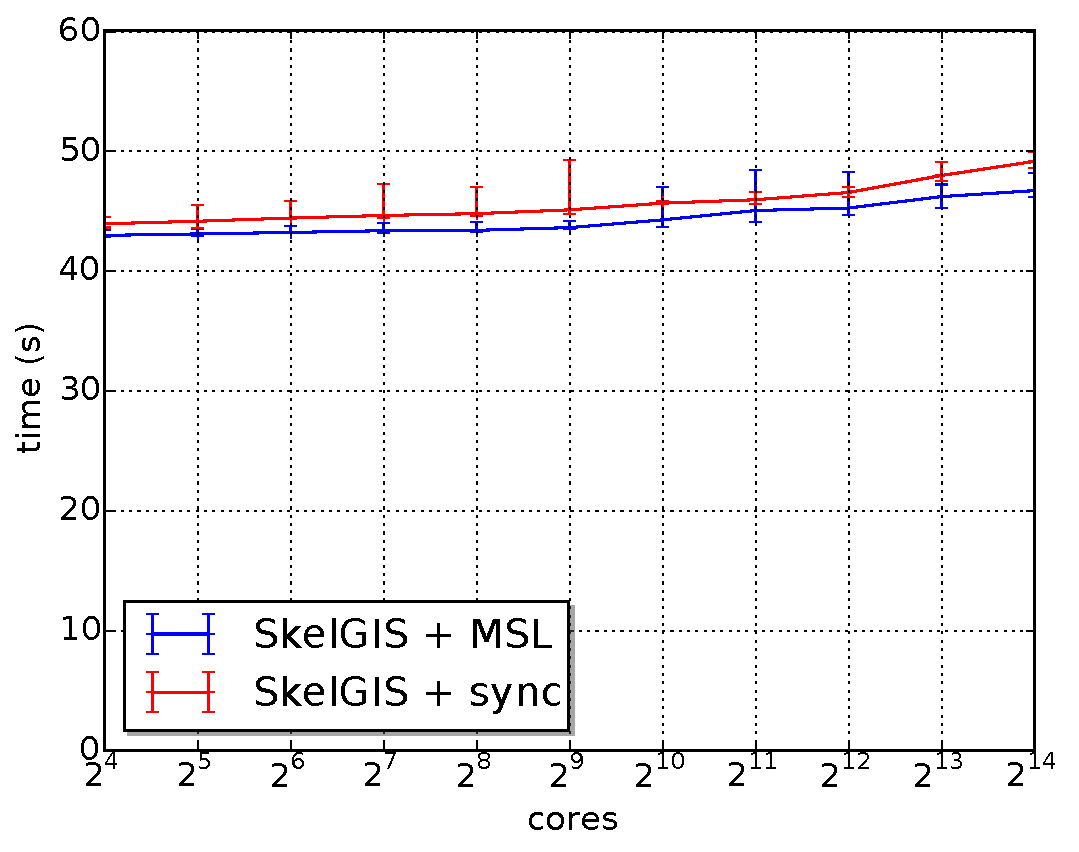
\includegraphics{../results/weak_scaling/400/median_weak.pdf}}
  \caption{weak-scaling 400x400 blocks.}
  \label{fig:mesh}
\end{center}\end{figure}

\begin{figure}[!h]\begin{center}
  \resizebox{8cm}{!}{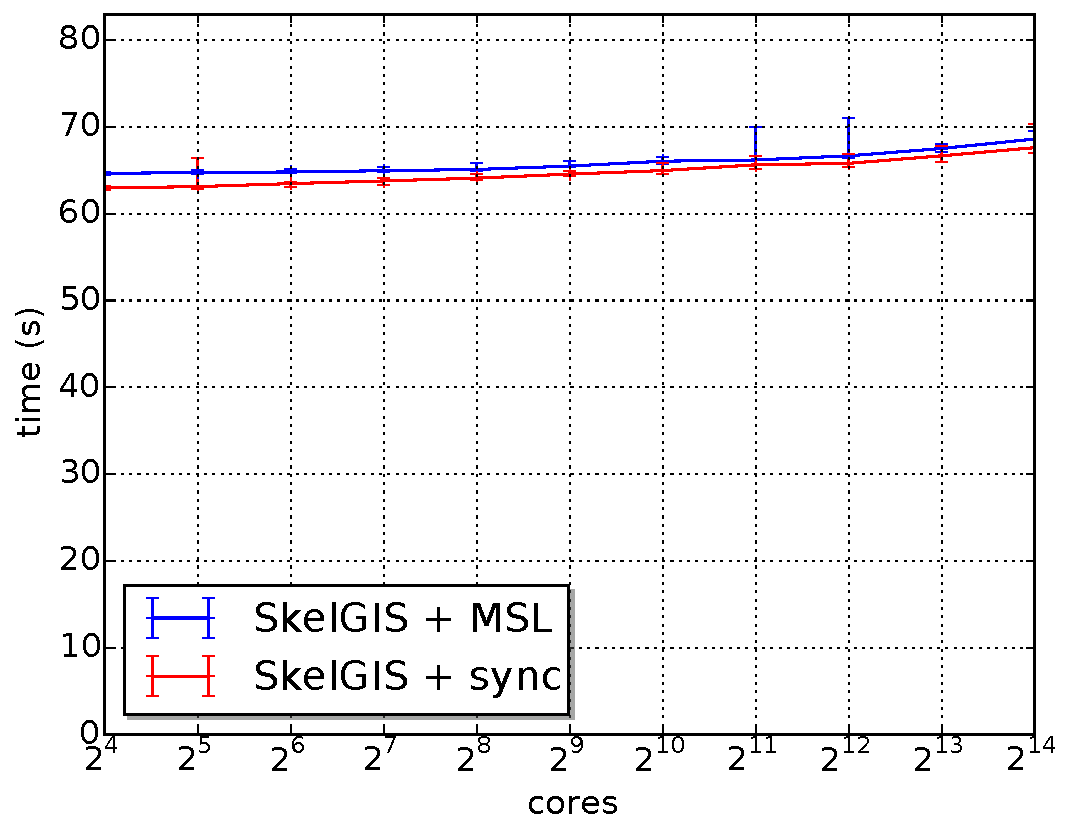
\includegraphics{../results/weak_scaling/800/median_weak.pdf}}
  \caption{weak-scaling 800x800 blocks}
  \label{fig:mesh}
\end{center}\end{figure}

\begin{figure}[!h]\begin{center}
  \resizebox{8cm}{!}{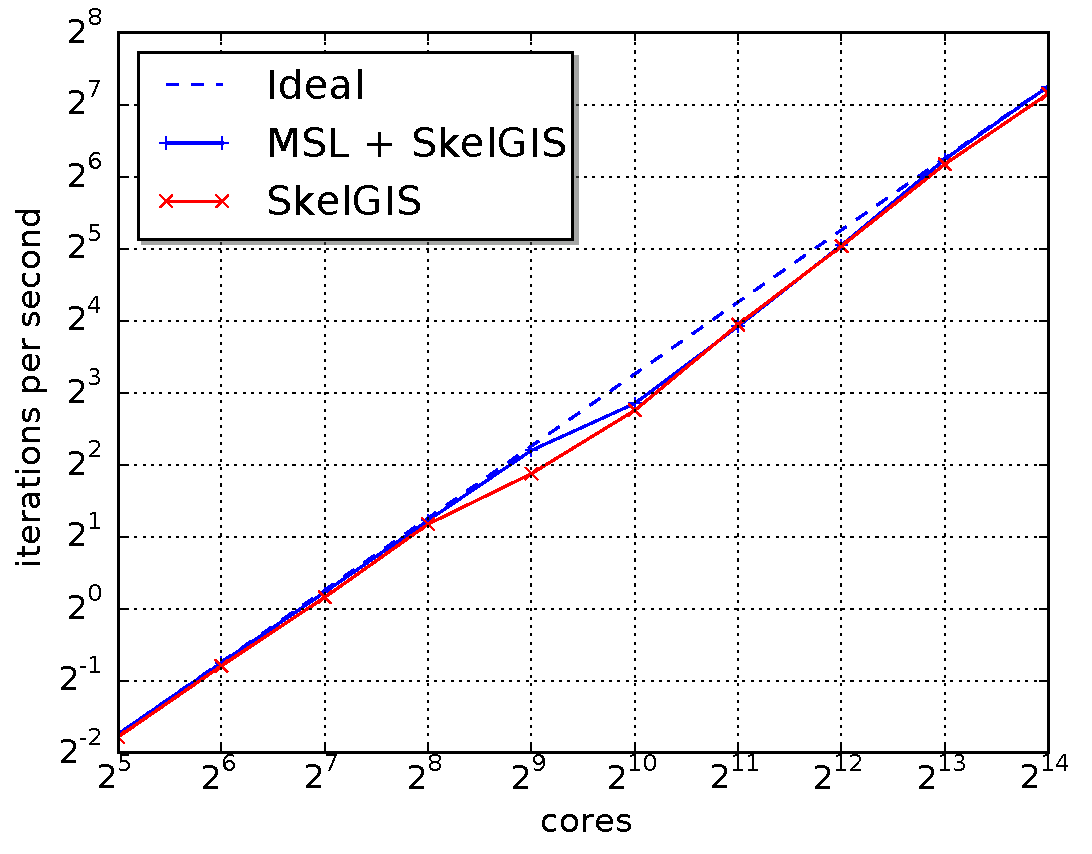
\includegraphics{../results/strong_scaling/10K_1K/median_strong.pdf}}
  \caption{strong-scaling 10kx10k, 1k iterations}
  \label{fig:mesh}
\end{center}\end{figure}

\item evaluation of the fusion

\begin{figure}[!h]\begin{center}
  \resizebox{8cm}{!}{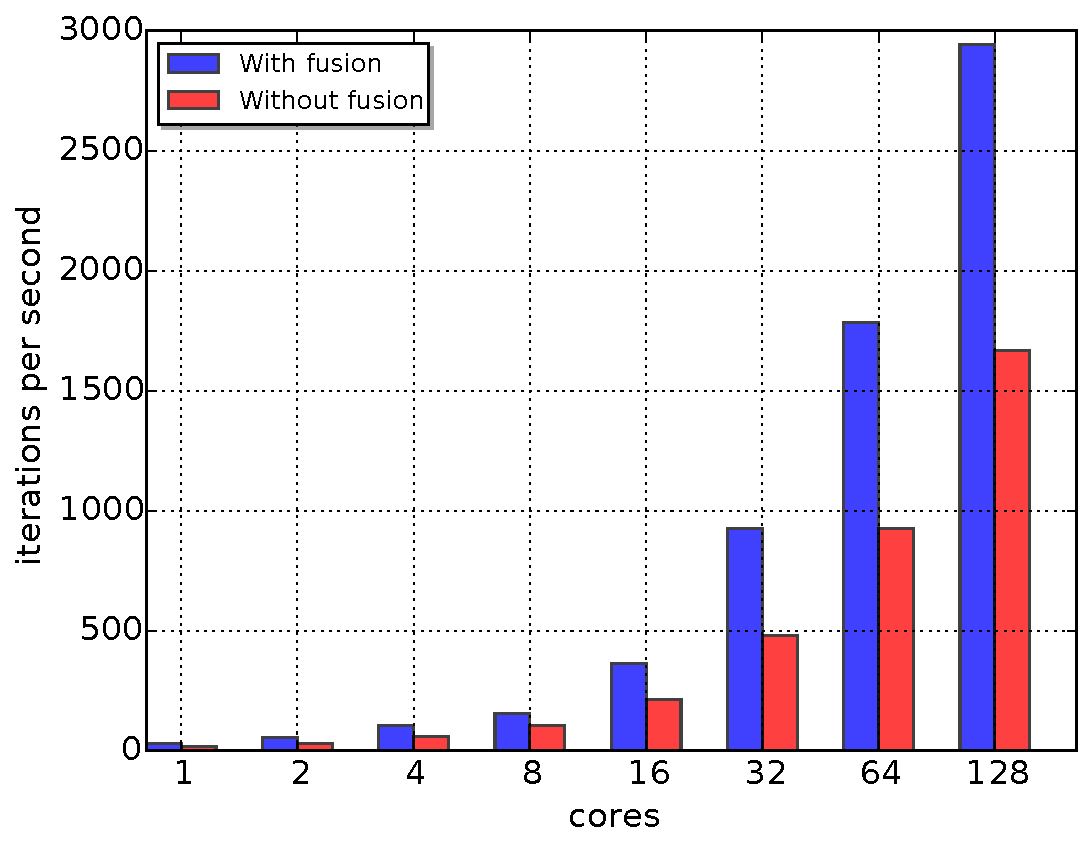
\includegraphics{../results/task_scaling/500_200/fusVSbase.pdf}}
  \caption{strong scaling 500x500, 200 iterations, with and without fusion}
  \label{fig:mesh}
\end{center}\end{figure}

\item evaluation of the hybrid parallelism

\begin{figure}[!h]\begin{center}
  \resizebox{8cm}{!}{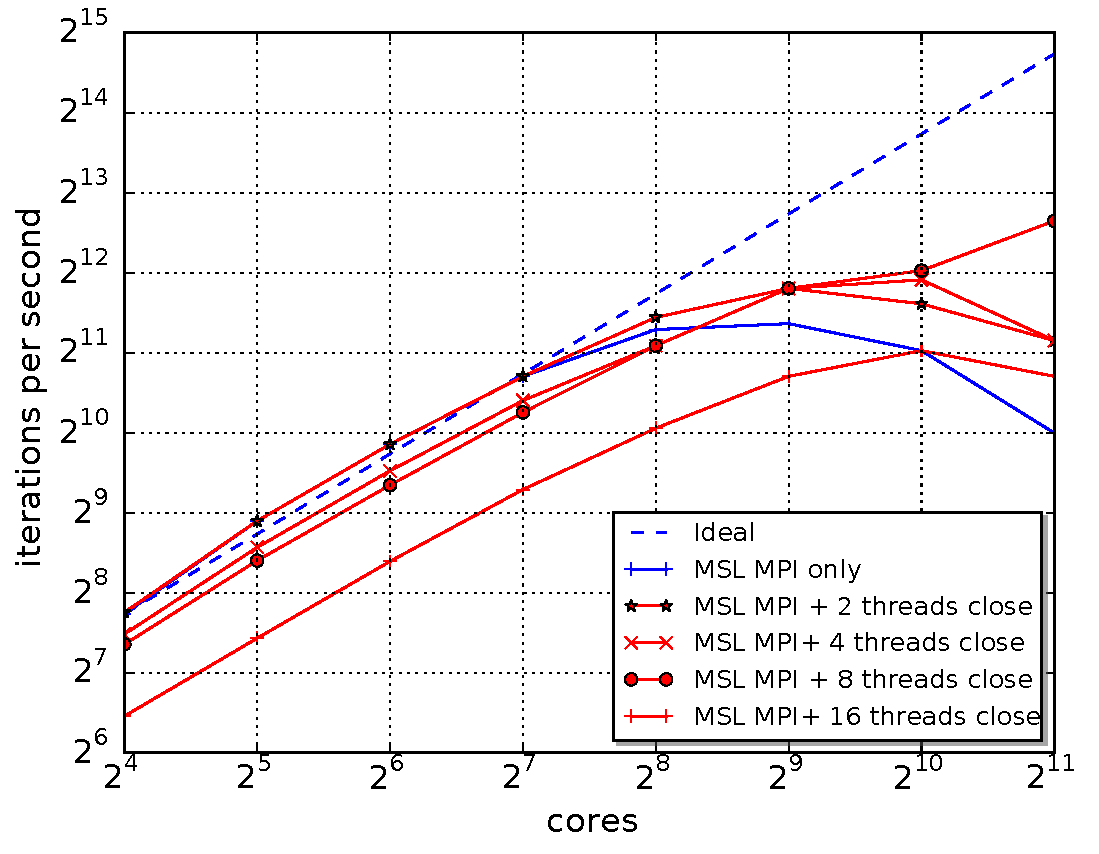
\includegraphics{../results/task_scaling/500_200/base_close_median.pdf}}
  \caption{MPI only vs MPI+threads with \emph{close} scheduling policy (OpenMP)}
  \label{fig:mesh}
\end{center}\end{figure}

\begin{figure}[!h]\begin{center}
  \resizebox{8cm}{!}{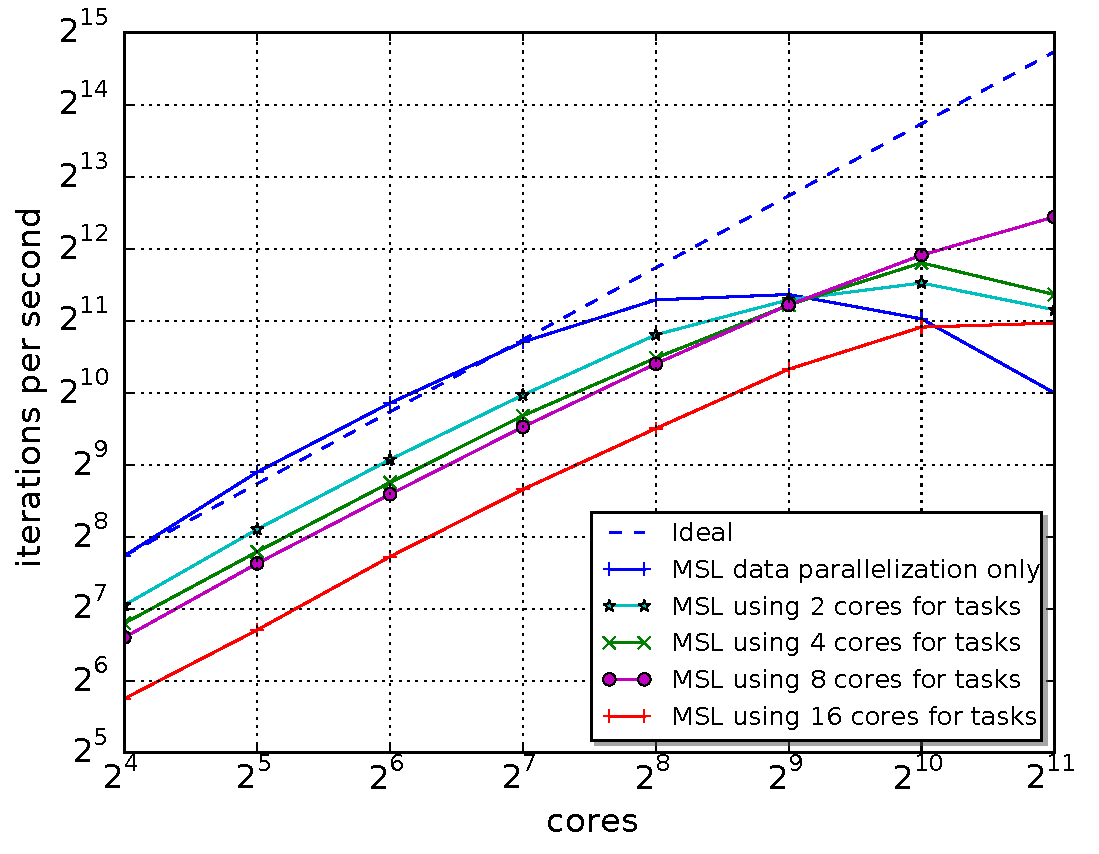
\includegraphics{../results/task_scaling/500_200/base_spread_median.pdf}}
  \caption{MPI only vs MPI+threads with \emph{spread} scheduling policy (OpenMP)}
  \label{fig:mesh}
\end{center}\end{figure}

\item analytic model for the results

\begin{figure}[!h]\begin{center}
  \resizebox{8cm}{!}{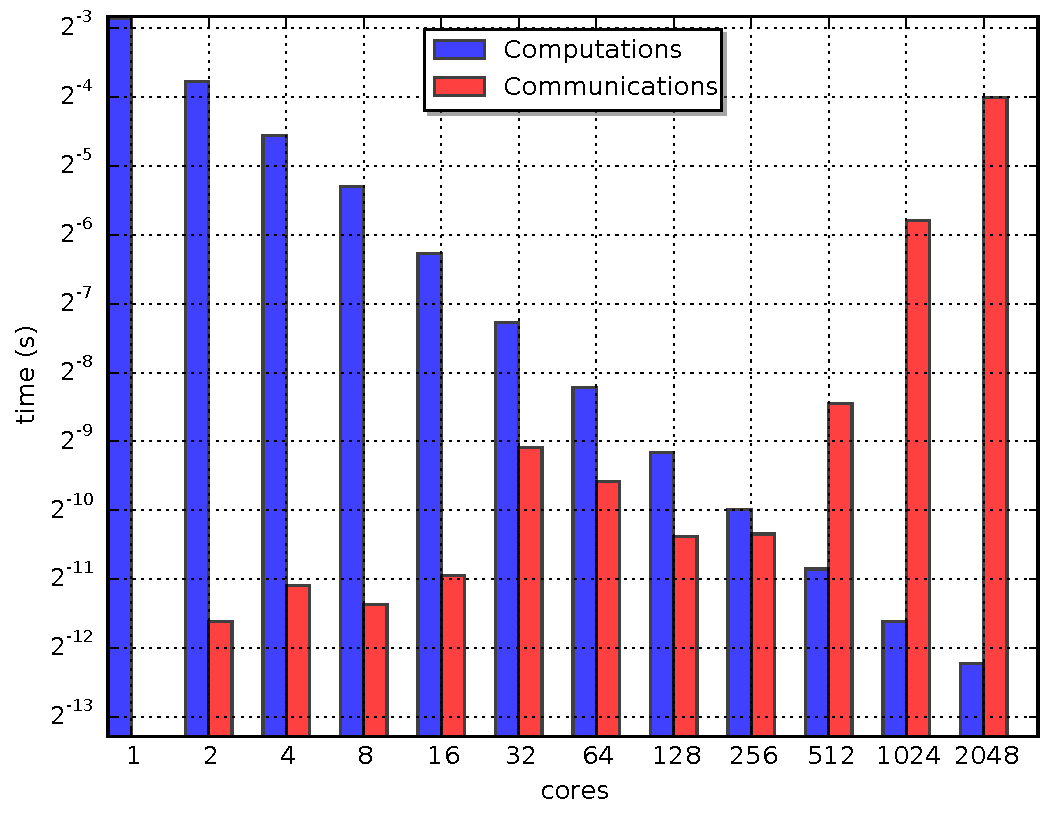
\includegraphics{../results/task_scaling/500_200/analytic/times.pdf}}
  \caption{Computation vs communication times in the MPI only application}
  \label{fig:mesh}
\end{center}\end{figure}

\end{itemize}
%------------------------------------------------------------------------------
\section{Related work}
\label{sect:rel}
\begin{itemize}
\item Lizst, Pochoir, PATUS for optimizations/parallelization of a single stencil kernel + mesh dependent
\item Halide for pipeline of stencil computations = mesh dependent
\item Reuse of external solutions as SkelGIS, GA, Lizst, Pochoir etc.
\end{itemize}
%------------------------------------------------------------------------------
\section{Conclusion}
\label{sect:concl}
%------------------------------------------------------------------------------

%\begin{acknowledgements}
%If you'd like to thank anyone, place your comments here
%and remove the percent signs.
%\end{acknowledgements}

\bibliographystyle{plain}
\bibliography{biblio}

\end{document}
% end of file template.tex

